%!TEX root = ../thesis.tex
%*******************************************************************************
%****************************** Second Chapter *********************************
%*******************************************************************************

\chapter{The SNO+ Detector}\label{chap:detector}
\epigraph{\textit{The light-soaked days are coming.}}{\textsc{John Green}}
\section{Detector Geometry}
% \nomenclature{\textbf{SNO}}{Sudbury Neutrino Observatory}
% \nomenclature{\textbf{UPW}}{Ultra-pure water}
\nomenclature{\textbf{AV}}{Acrylic vessel}
\nomenclature{\textbf{PSUP}}{PMT support structure}
\nomenclature{\textbf{PMT}}{Photomultiplier Tube}
\nomenclature{\textbf{OWLs}}{Outward-looking PMTs}
The SNO+ detector is a large, multi-purpose neutrino detector built in the SNOLAB underground laboratory near Sudbury, Canada. The main detector structure is taken from the Sudbury Neutrino Observatory (SNO)~\cite{BOGER2000172}, % cite
which can be seen in Fig.~\ref{fig:snoplus_detector}. 
SNO+ is an optical detector: light is generated within a central spherical detector medium, with those photons being detected by an array of 9362 inward-facing Photomultiplier Tubes (PMTs). The properties of physics events are then estimated by looking at the number of photons that were detected, as well as their timing and spatial distributions. Because of this, the detector must be optimised to achieve a high, stable, and well-understood detection efficiency of photons, as well as a timing resolution of detected photons $\mathcal{O}(\SI{1}{\ns})$. A more detailed description of how physics events get detected in SNO+ is given in Section~\ref{sec:event_journey}.

The main detector medium of SNO+ changes depending on the phase of the experiment; specifics are given in Section~\ref{sec:exp_phases}. This medium is held within a \SI{12}{\metre} diameter sphere known as the Acrylic Vessel (AV). The AV floats within a body of ultra-pure water (UPW), beyond which is a stainless steel support structure (PSUP) that holds the PMTs. The AV is kept in place relative to the PSUP through a series of `hold-up' and `hold-down' tensylon ropes. All of these components are suspended within a large cylindrical cavity also filled with UPW. 91 outward-looking PMTs (OWLs) are also affixed to the outside of the PSUP, allowing for the effective vetoing of cosmic ray muons.

Directly above the detector is the Deck, upon which all the detector electronics are kept. Access within the AV for calibration tools and filling is possible through the acrylic `neck' on top of the AV. Full details of the design of the current detector can be found in~\cite{albaneseSNOExperiment2021}.

\begin{figure}
    \centering
    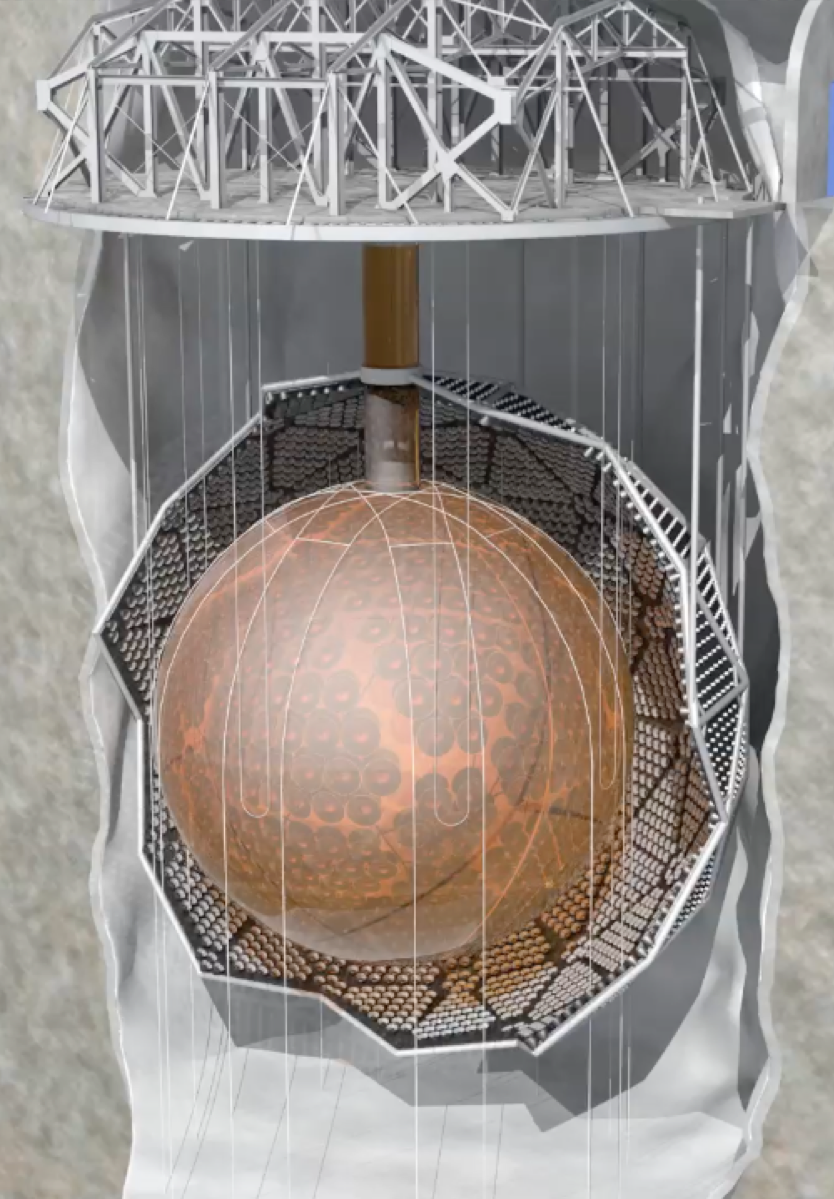
\includegraphics[width=0.48\linewidth]{2_Detector/Figs/detector_picture.png}
    \caption[3D model of the SNO+ detector]{3D model of the SNO+ detector~\cite{albaneseSNOExperiment2021}.}
    \label{fig:snoplus_detector}
\end{figure}

\section{Experimental Phases}\label{sec:exp_phases}
\nomenclature{\textbf{LAB}}{Linear alkylbenzene}
\nomenclature{\textbf{PPO}}{2,5-Diphenyloxazole}
\nomenclature{\textbf{Bis-MSB}}{1,4-Bis(2-methylstyryl)benzene}
\nomenclature{\textbf{DDA}}{N,N-Dimethyldodecylamine}
\nomenclature{\textbf{BD}}{1,2-Butanediol}
\nomenclature{\textbf{TeA}}{Telluric acid, \ce{Te(OH)_{6}}}
\nomenclature{\textbf{TeLS}}{Tellurium-loaded liquid scintillator}
\nomenclature{\textbf{BHT}}{Butylated hydroxytoluene}
SNO+ was designed to fulfil a number of physics goals over multiple `phases' of the detector's lifetime. The phases are distinguished by the medium that fills the AV. The first main phase (after a brief \textbf{Air Fill Phase} used only for detector commissioning) was that of the \textbf{Water Fill Phase}, with data taken between May 2017 and July 2019. This was used to perform fundamental optical calibrations of the detector~\cite{andersonOpticalCalibrationSNO2021}, % Water optics paper
measurements of the solar neutrino flux~\cite{andersonMeasurementSolarNeutrino2019}, % water solar papers
observation of neutrino oscillations in reactor anti-neutrinos~\cite{allegaEvidenceAntineutrinosDistant2023}, % water antinu paper
and searches for nucleon decay~\cite{andersonSearchInvisibleModes2019,allegaImprovedSearchInvisible2022}. %nucleon decay papers

After this, the detector was filled with 780 tonnes of a type of liquid scintillator known as linear alkylbenzene (LAB), mixed with the fluor 2,5-diphenyloxazole (PPO). More information on the physics of scintillators can be found in Section~\ref{sec:interactions_w_matter}. Filling of the LAB-PPO cocktail had to be paused in March 2020 due to the COVID-19 pandemic, leading to the detector having its bottom half still filled with UPW, and the top half filled with LAB and PPO at \SI{0.5}{\gpl}. This impromptu phase became known as the \textbf{Partial Fill}, and allowed for some creative analyses to be performed: an initial neutrino oscillation analysis from reactor anti-neutrinos~\cite{morton-blakeFirstMeasurementReactor2021}, % Iwan's thesis & forthcoming paper
as well as the first ever observation of directionality in a high light yield scintillator~\cite{allegaEventbyEventDirectionReconstruction2023,patonDirectionalReconstructionLiquid2023}. % Josie's thesis & forthcoming PRL
Eventually, filling of the detector with liquid scintillator completed in May 2021. At that point, the concentration of PPO in the detector was at \SI{0.6}{\gpl}, markedly below the target level of \SI{2.0}{\gpl}. A further `PPO top-up' campaign then proceeded, finishing in April 2022 with a final concentration of \SI{2.2}{\gpl} PPO. Thus began the \textbf{Scintillator Phase} of the experiment, which continues on during the time of writing. The main goals for this phase include a number of solar neutrino analyses (including the one described in Chapter~\ref{chap:solar_osc_analysis}), a precision measurement of the neutrino oscillation parameter \dmsq{} using reactor anti-neutrinos~\cite{morton-blakeFirstMeasurementReactor2021}, % Iwan's thesis
further calibrations of the detector, and measurements of the various backgrounds.

Two further chemicals are being added to the scintillator cocktail at the time of writing. The antioxidant butylated hydroxytoluene (BHT) has been added in July 2023 to capture any free-radicals within the liquid scintillator, hopefully preventing any oxidation reactions that could lead to the `yellowing' of the scintillator, a degradation of its optical properties. The addition of BHT is not expected to directly impact the detector's optics in any substantial way. However, the other substance to also be added, 1,4-Bis(2-methylstyryl)benzene (bis-MSB), will impact the optics. Bis-MSB acts as a `wavelength-shifter' which enables the scintillator cocktail to transmit light with a greater overall detection efficiency --- more on the details of this in Section~\ref{sec:scintillation}.

Finally, in the near future the detector will be loaded with Tellurium for the \textbf{Tellurium Phase}, allowing for the flagship analysis of the experiment to begin: neutrinoless double beta decay. In order to load Te within the liquid scintillator in a stable manner, a chemical loading process has been developed, as described in~\cite{autyMethodLoadTellurium2023}. % Te loading paper
The Te starts within \ce{Te(OH)_{6}} (telluric acid, otherwise known as TeA), which after purification will be reacted with 1,2-butanediol (BD) via heating and addition of N,N-Dimethyldodecylamine (DDA), which acts as a stabiliser. What results is tellurium-loaded scintillator, TeLS.


% \begin{itemize}
%     \item Describe the SNO+ geometry at a high level: explain structure, and why certain design choices were made.
%     \item Describe standard coordinate axis; note AV offset.
%     \item Mention the main phases of SNO+, both past, present, and future.
% \end{itemize}
\section{Detecting and Recording an Event in SNO+: A Journey}\label{sec:event_journey}
To understand the SNO+ detector well, it is worth thinking about how the information contained in a physics event, e.g. a solar neutrino interaction, gets observed. This section follows the journey of such an event.
\subsection{Particle Interactions with Matter}\label{sec:interactions_w_matter}
All observable physics events within the detector begin by the generation of some form of ionising radiation: $\alpha$, $\beta^{\pm}$, $p$, $\mu$ or $\pi$. These can be created via numerous processes, both exciting (e.g. \onbb{} or interactions of neutrinos) and annoying (e.g. decay of background radioisotopes): see Section~\ref{sec:background_processes} for some of them. Regardless of their origin, these particles begin propagating through the detector, and interacting with the detector medium. A number of mechanisms then allow for the generation of optical-wavelength light as a result of these interactions.
\subsubsection{Cherenkov Light Emission}
Whenever a charged particle travels through a dielectric medium at speeds faster than the speed of light in that medium, light is generated from the `wake' of induced dipoles. This is known as \textbf{Cherenkov light}, a process much akin to the `sonic boom' that occurs when an object travels at supersonic speeds through a medium. This light emanates outwards in a cone along the direction of the charge's travel; the angle of the cone $\theta_{\gamma}$ being purely a function of the speed of the charged particle relative to the speed of light in vacuum, $\beta$, and the refractive index of the medium $n(\omega)$ at a given frequency $\omega$: $\cos{\theta_{\gamma}}(\omega) = \frac{1}{n(\omega)\beta}$. There is then a minimum speed necessary for Cherenkov light to be generated: $\beta_{\textrm{min}}(\omega) = 1/n(\omega)$.

In addition to the characteristic cone shape of the light, the spectrum of the light generated is also distinctive. Igor Tamm and Ilya Frank determined the expected energy $dE$ emitted per unit length travelled by the charged particle, $dx$, as~\cite{frankCoherentVisibleRadiation1937}: % Frank-Tamm formula
\begin{equation}
    \frac{dE}{dx} = 
    \frac{q^2}{c^{2}}\int_{\beta n(\omega)>1}\omega\left(1-\frac{1}{\beta^{2}n^{2}(\omega)}\right)d\omega.
\end{equation}
Here, $q$ is the charge of the moving particle. The Cherenkov emission spectrum during the water phase is shown in the black dotted line of Fig.~\ref{fig:cherenkov_scintillator_abs_emit_dist}.

\begin{figure}
    \centering
    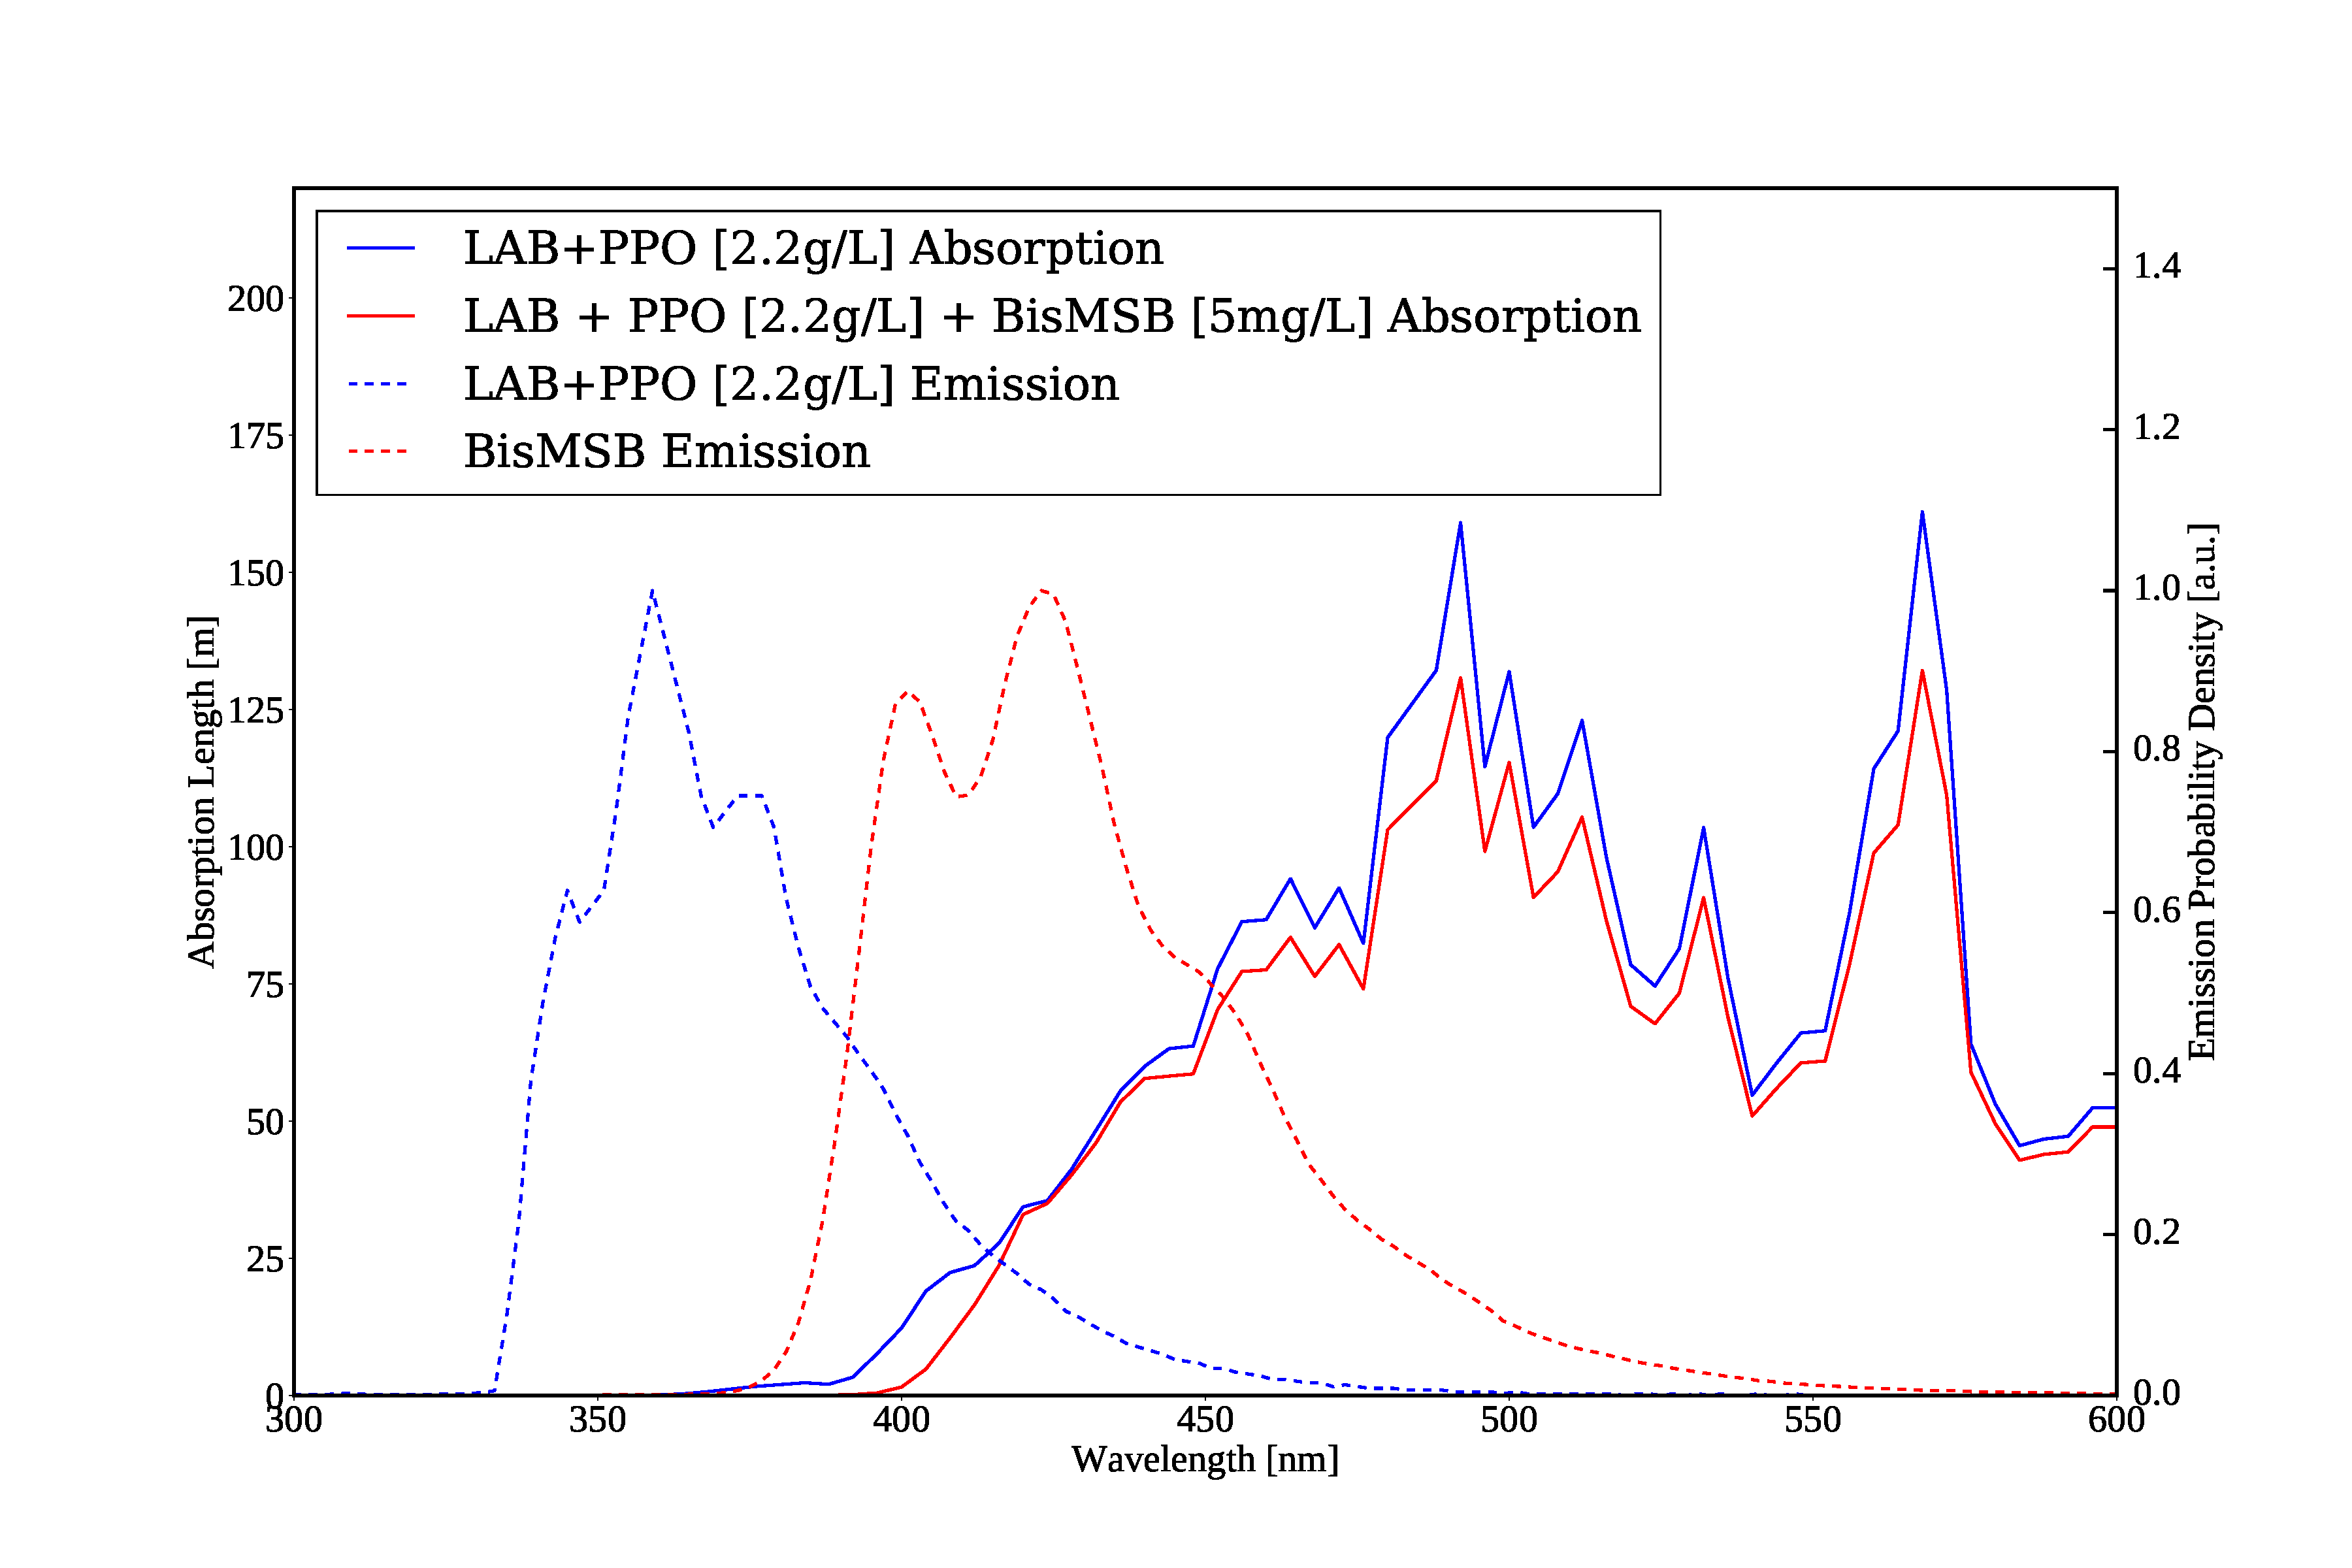
\includegraphics[width=0.8\linewidth]{2_Detector/Figs/scint_lengths_LABPPOBisMSB_plot_nice.pdf}
    \caption[Comparison of the SNO+ detector media's emission properties, versus optical phase]
    {Comparison of the SNO+ detector media's emission and absorption properties, versus optical phase~\cite{kaptanogluOpticsOverviewProposed2016,kaptanogluDocumentationAttenuationStudies2022}. % cite optics?
    }
    \label{fig:cherenkov_scintillator_abs_emit_dist}
\end{figure}

All SNO+ detection media allow Cherenkov light to be generated, as long as sufficiently high energy particles traverse it. In the water fill phase of the detector, Cherenkov light was the only means by which light could be generated. Light from Cherenkov emission can still be created in liquid scintillator, but it tends to be swamped by another form of light generation: scintillation.
\subsubsection{Scintillation}\label{sec:scintillation}
For certain special classes of material, the excitation and ionisation of atoms nearby a moving charged particle can lead to the generation of optical-wavelength light, in a process known as \textbf{scintillation}. Although multiple varieties of scintillator exist, the one used in SNO+ is that of an organic liquid scintillator. For such liquids, scintillation light is generated from the de-excitation of delocalised electrons within carbon--carbon `$\pi$-bonds'~\cite{birksChapterScintillationProcess1967}. A major example of these $\pi$-bonds are found in benzene rings, which are present in LAB, PPO, and bis-MSB.

Because of this delocalised structure, excited atomic $\pi$-electrons can stay in what is typically the first-excited state for somewhat longer than typical excited states: lifetimes of $\mathcal{O}(\SI{e-9}{\second})$ as opposed to $\mathcal{O}(\SI{e-12}{\second})$. This is what gives scintillation light its characteristic `slow' response relative to the instantaneous light generated by the Cherenkov process. Moreover, decays from this state can emit light typically in the optical-wavelength range. 
$\pi$-electrons can end up in the first-excited state either by direct excitation, or by ionisation followed by recombination. Because the ground state of these electrons are spin-singlet states, atomic spin selection rules~\cite{birksChapterScintillationProcess1967} strongly prefer any direct excitations to stay in a spin-singlet state. As a result, so-called ``inter-system crossing'' from an excited singlet state to an excited triplet state is strongly suppressed.
% In addition to excited electrons, ionised electrons can also recombine --- that is, re-enter atomic orbitals --- into various excited states, and then decay back to the ground state, also allowing for the possibility of scintillation light to be generated.

% Because of atomic spin selection rules~\cite{birksChapterScintillationProcess1967}, % cite something!
% scintillation light typically has, at the very least, a `fast' and `slow' time component.
However, ionised electrons that recombine have no such restriction, and so readily form excited triplet states. Once in such a state, the same spin selection rules strongly suppress the decay of these excited triplet electrons back down to the singlet ground state. This leads to scintillation light having, at the very least, a `fast' and `slow' time component. In SNO+, we currently model emission of scintillation light from LAB-PPO with 4 time components, following the timing distribution $f(t)$ given by:
\begin{equation}
    f(t) = \sum_{i}A_{i}\left(\frac{e^{-t/\tau_{i}}-e^{-t/\tau_{\mathrm{rise}}}}{\tau_{i}-\tau_\mathrm{rise}}\right),\; t > 0.
\end{equation}
Here, $A_{i}$ and $\tau_{i}$ correspond to the fraction of light emitted and decay constant for each component respectively, and $\tau_\mathrm{rise}$ is a common rise time. The current values for these parameters used in simulations for the emission from electron tracks can be seen in Table~\ref{tab:scint_reem_params}. These were obtained by Rafael Hunt-Stokes through the fitting of tagged \ce{^{214}Bi} $\beta$-decay events within the detector with \SI{2.2}{\gpl} LAB-PPO~\cite{hunt-stokesEmissionTimingTuning2022}. A plot from R. Hunt-Stokes showing this fit between data and simulation is shown in Fig.~\ref{fig:typical_tres_dist_physics}.

\begin{table}[!th]
    \centering
    \begin{tabular}{c p{2cm} p{2cm}}
        \hline
        Component & $A_{i}$ & $\tau_{i}$ [ns] \\ \hline \hline
        1         & 0.665   & 7.35  \\
        2         & 0.218   & 5.45  \\
        3         & 0.083   & 117.5 \\
        4         & 0.0346  & 425   \\
        Rise      & --      & 0.8   \\
        \hline
    \end{tabular}
    \caption[Current values used to model scintillator emission from electrons in \SI{2.2}{\gpl} LAB-PPO]
    {Current values used to model scintillator emission from electrons in \SI{2.2}{\gpl} LAB-PPO~\cite{latorreNewMeasurementsTiming2016,hunt-stokesEmissionTimingTuning2022}.}
    \label{tab:scint_reem_params}
\end{table}

\begin{figure}[!th]
    \centering
    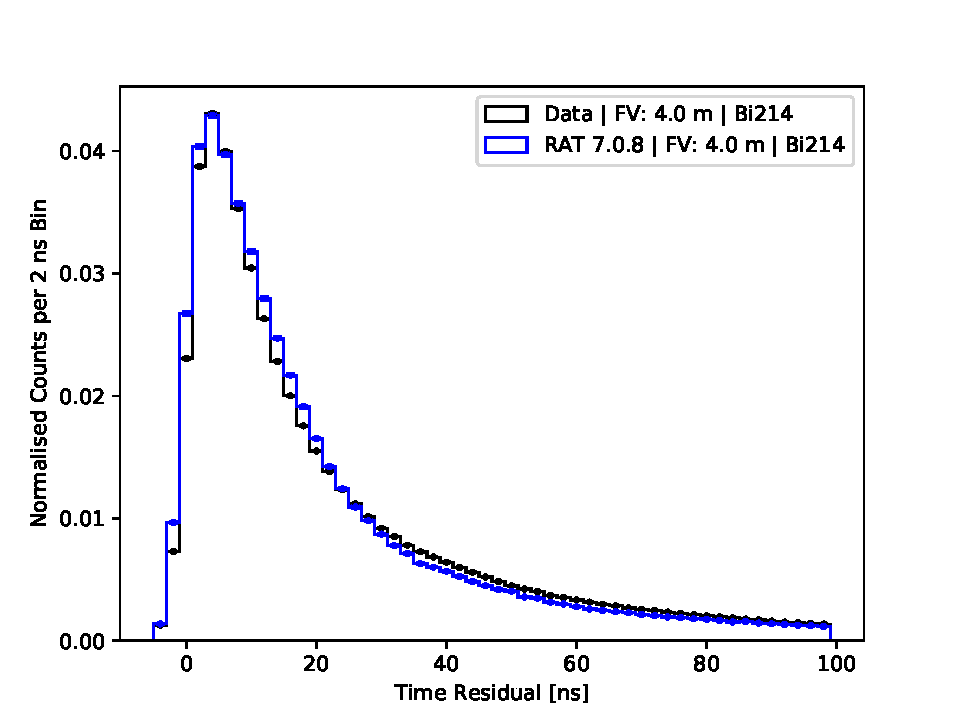
\includegraphics[width=0.8\linewidth]{2_Detector/Figs/daniel_old_tuning_250Cut_2ns.pdf}
    \caption[Comparison between the observed emission time of \ce{^{214}Bi} $\beta$-decays in data versus MC]
    {Comparison between the observed emission time distribution of electrons from tagged \ce{^{214}Bi} $\beta$-decays and a production of matching simulated events, after fitting the timing constants. Adapted from~\cite{hunt-stokesEmissionTimingTuning2022}.% 
    ``FV'' corresponds to the Fiducial Volume used in this plot; ``RAT 7.0.8'' is the version of the simulation software used to compare to data.
    }
    \label{fig:typical_tres_dist_physics}
\end{figure}

In SNO+, a separate scintillating component, PPO, has been added to the LAB. When an LAB molecule is excited, that energy can be transferred to a PPO molecule through what is known as a `non-radiative transfer'. In short, this transfer of energy occurs not through the emission and absorption of optical photons, but through the coupling of the molecules' electric dipoles during a collision. The now-excited PPO molecule can then de-excite to emit scintillation light. The additional pathway that PPO provides substantially increases the light yield of the scintillator.

The compound bis-MSB is also being added to the scintillator cocktail at the time of writing. This is a `wavelength-shifter': scintillation light at short wavelengths is absorbed, and then re-emitted at longer wavelengths, where the detection efficiency of the PMTs is greatest ($\sim\SI{420}{\nm}$). More on the properties of the PMTs in SNO+ can be found in Section~\ref{sec:pmts}. This shift in wavelength further boosts the measured light yield of the scintillator within the detector. The net effect of the three scintillating components within SNO+ can be seen in Fig.~\ref{fig:cherenkov_scintillator_abs_emit_dist}. Note how, as energy is transferred from one scintillation component to another, the wavelength of light emitted gets necessarily longer as energy is lost to heat.

The light yield of a scintillator, i.e. the amount of optical photons generated per unit of energy deposited into the scintillator, is a function not just of the scintillator but also the incident particle's ionisation strength. In particular, $\alpha$ particles are far more effective at exciting and ionising nearby atoms, and so can deposit far more of its energy into the scintillator per unit volume. However, the strength of this ionisation for $\alpha$s can actually become at detriment to the generation of scintillation light. Empirically, scintillators follow to first order Birks' Law for their scintillation light yield~\cite{birksChapterScintillationProcess1967a}: % Birks Law ref.
\begin{equation}
    \frac{dL}{dx} = S\frac{\frac{dE}{dx}}{1+k_{\mathrm{Birks}}\frac{dE}{dx}},
\end{equation}
where $\frac{dL}{dx}$ is the number of photons emitted per unit track length, $\frac{dE}{dx}$ is the energy loss of the incident particle per unit track length, $S$ is the scintillator's characteristic light yield constant, and $k_{\mathrm{Birks}}$ is the scintillator's ``Birks' Constant''. In the \SI{2.2}{\gpl} LAB-PPO scintillator currently within SNO+, $S$ and $k_{\mathrm{Birks}}$ are measured to be approximately \SI{14000}{\gamma\per\MeV} and \SI{0.077}{\mm\per\MeV}, respectively~\cite{riccettoRATOptics2g2022}. % cite where we got S and kb values from.
For minimum-ionising particles such as a \SI{6}{\MeV} electron $\frac{dE}{dx}\approx\SI{2}{\MeV\per\cm}$~\cite{workmanReviewParticlePhysics2022a}, % cite PDG?
meaning the denominator of this equation is close to 1, and so the amount of scintillation light generated is just $\frac{dL}{dx} \approx S\cdot\frac{dE}{dx}$. However, for $\alpha$-particles generated in radioactive decays, this denominator can become substantial. For example, $\alpha$-particles are generated at \SI{5.304}{\MeV} from the decays of \ce{^{210}Po} nuclei~\cite{kondevNuclearDataSheets2008}. However, these events generate light equivalent to a \SI{0.45}{\MeV} event in the detector.


\subsection{Optical Processes}\label{sec:optical_processes}
Once optical-wavelength photons have been created within the detector, various processes can then occur that can hinder their path towards a PMT, and therefore modify the observed signal. This subsection covers the main optical processes, with a focus on Rayleigh scattering, as an understanding of this phenomenon is critical for Chapters~\ref{chap:smellie_hardware}--\ref{chap:smellie_analysis}.

\subsubsection{Rayleigh Scattering}
Optical scattering is the general process of how light is scattered by particles within a medium. This is fundamentally an electrodynamical process: an electromagnetic wave is incident on the set of particles within the medium, which induces these particles to oscillate within the field, and therefore generates their own electromagnetic radiation in response. Usually, this `scattered' radiation has the same frequency as that of the incident radiation, and therefore the scattering is said to be \textit{elastic}. It is possible under certain circumstances for this scattered radiation to be of a different wavelength than the incident radiation: in which case, the scattering was \textit{inelastic}. However, this latter type of scattering, also known as Raman scattering, occurs negligibly in SNO+.

The simplest form of elastic optical scattering is known as \textit{Rayleigh scattering}, after the initial formulation by Lord Rayleigh~\cite{rayleighTransmissionLightAtmosphere1899}, and relies on the following assumptions of a system of particles:
\begin{itemize}
    \item the particles are an ideal gas, i.e. there are negligible inter-molecular forces;
    \item the particles are spherical;
    \item the particle radii are much less than the wavelength of the incident light;
    \item the induced dipole moments of the particles can be established on a timescale much less than the period of the electromagnetic wave.
\end{itemize}
If the latter two assumptions are lifted, one ends up with the more general \textit{Mie Theory}, first described by Gustav Mie~\cite{mieContributionsOpticsTurbid1908} % ref Mie theory paper
and Ludvig Lorenz~\cite{lorenzLumiereReflechieRefractee1898}. % Lorenz's paper

The optical media within SNO+ are all liquids or solids, and so the first assumption above of negligible inter-molecular forces does not at all hold. A different theory was developed by Einstein~\cite{einsteinTheoryOpalescenceHomogeneous1910}, %
Smoluchowski~\cite{smoluchowskiMolecularKineticTheory1908}, %
and Cabannes~\cite{cabannesRelationshipDegreePolarisation1920}, %
in which light scatters off of the local charge density fluctuations that naturally are present in a medium because of the thermal motion of molecules. This theory predicts that the \textit{Rayleigh ratio} $R$, the fraction of the incident light that gets scattered at a \ang{90} angle, per unit volume per unit solid angle, is given by~\cite{zhangEstimatingScatteringPure2009}:
\begin{equation}
    R = \frac{\pi^{2}}{2\lambda^{4}}\left[\rho\left(\frac{\partial\varepsilon}{\partial\rho}\right)_{T}\right]^{2} k_{B}T \kappa_{T}\frac{6+6\delta}{6-7\delta}.
\end{equation}
Here, $\rho$ is the density of the medium, $\left(\frac{\partial\varepsilon}{\partial\rho}\right)_{T}$ is the partial derivative of the dielectric constant $\varepsilon$ with respect to a changing density assuming a constant temperature $T$, $k_{B}$ is the Boltzmann Constant, $\kappa_{T}$ is the medium's isothermal compressibility, and $\delta$ is the \textit{depolarisation ratio} of the medium. This latter variable describes how anisotropic the medium's electric polarisability is --- a medium with no anisotropy in the polarisability has $\delta = 0$. The $1/\lambda^{4}$ dependence indicates that short wavelengths of light will get scattered to a far greater extent than longer wavelengths.

Various alternative versions of this formula exist, converting $\rho\left(\frac{\partial\varepsilon}{\partial\rho}\right)_{T}$ into something more straightforward to measure via use of thermodynamical or empirical equations --- see~\cite{zhangEstimatingScatteringPure2009,jiangbotimzhaoImprovedSpectrophotometricMethod2020} for discussions. Also, in liquid mixtures, the total observed scattering can substantially exceed what would be expected from the sum of the individual components. This is because fluctuations in the dielectric constant can also be caused by fluctuations in the relative composition of the medium in a given volume element~\cite{coumouIsotropicLightscatteringBinary1964,kirkwoodLightScatteringArising1950}.

Although $R$ is the scattering quantity most easy to measure in bench-top laboratory experiments, for SNO+ two different properties are more relevant. The main observable is a material's \textit{Rayleigh scattering length}, $l_{\textrm{Ray}}$: the mean distance a photon is expected to travel before Rayleigh scattering. One can show that the Rayleigh scattering length is given by~\cite{zhouRayleighScatteringLinear2015}: % https://arxiv.org/pdf/1504.00987.pdf
\begin{equation}
    l_{\textrm{Ray}} = \left[\frac{8\pi}{3}\frac{2+\delta}{1+\delta}R\right]^{-1}.
\end{equation}
The other important feature of Rayleigh scattering is its angular dependence. The scattered intensity as a function of the scattered angle, $I(\theta)$, has an equation of the form:
\begin{equation}
    I(\theta) \propto \left(1+\frac{1-\delta}{1+\delta}\cos^{2}\theta\right).
\end{equation}

% The general solution to elastic optical scattering was first described by Gustav Mie~\cite{mieContributionsOpticsTurbid1908} % ref Mie theory paper
% and Ludvig Lorenz~\cite{lorenzLumiereReflechieRefractee1898} % Lorenz's paper
% in what is now known as \textit{Mie Theory}. In this theory, it is assumed that a plane wave of wavelength $\lambda$ is incident on a dielectric sphere of radius $a$. While the general solution to the problem of Mie scattering is somewhat complicated, in certain regimes one can make further simplifying assumptions that substantially reduce the complexity of the result. In particular, if one assumes that the size of the particle is much smaller than the wavelength of light, and that any induced dipole moment can actually be established in the time window allowed by the oscillation period of the electromagnetic field~\cite{HulstH.C.vande1981Lsbs}, % Rayleigh criteria
% then one can obtain \textit{Rayleigh scattering}. This simpler case is so-called because of its initial formulation by Lord Rayleigh~\cite{rayleighTransmissionLightAtmosphere1899}. % Rayleigh's scattering paper

% One can show that the differential cross-section associated with Rayleigh scattering of unpolarised light off a single particle, $\frac{d^{2}\sigma_{\textrm{Ray}}}{d\theta d\phi}\left(\theta,\phi\right)$, is given by~\cite{jacksonSection10Scattering1998}: % cite something that gets rayleigh scattering formula
% \begin{equation}
%     \frac{d^{2}\sigma_{\textrm{Ray}}}{d\theta d\phi}\left(\theta,\phi\right) = \frac{8\pi a^{6}}{\lambda^{4}}\left(\frac{n_{\textrm{par}}^{2}-1}{n_{\textrm{par}}^{2}+2}\right)^{2} \left(1+\cos^{2}\theta\right).
% \end{equation}
% Here, $\theta$ and $\phi$ correspond respectively to the polar and azimuthal angles of the scattered waves relative to the incoming wave, and $n_{\mathrm{par}}$ is the refractive index of the scattering particle. Most important to notice about this equation is that the cross-section follows a strong $1/\lambda^{4}$ dependence, meaning that short wavelengths of light will be scattered to far greater extents than that of longer wavelengths. Secondly, the light is not scattered isotropically, but according to a $1+\cos^{2}\theta$ dependence. This means that most light is either scattered directly forwards or backwards, and little gets scattered orthogonally to the direction of the incident light. This is useful when it comes to trying to measure scattering in the SNO+ detector, as it provides a handle upon which to distinguish scattered light from isotropically-emitted scintillation light.

% Of course, what matters is the scattering that occurs within an entire bulk medium, not just the scattering off of a single molecule. From a macroscopic perspective, the key quantity of interest is a material's \textit{Rayleigh scattering length}, $l_{\textrm{Ray}}$: the mean distance a photon is expected to travel before Rayleigh scattering. One can show that, assuming the above differential scattering cross-section, the Rayleigh scattering length is given by~\cite{zhouRayleighScatteringLinear2015}: % https://arxiv.org/pdf/1504.00987.pdf
% \begin{equation}
%     l_{\textrm{Ray}} = \left[\frac{16\pi}{3}R\right]^{-1}.
% \end{equation}
% $R$ is the \textit{Rayleigh ratio}, $R=\frac{1}{V}\frac{d^{2}\sigma_{\textrm{Ray}}\left(\ang{90}\right)}{d\theta d\phi}$, where $V$ is the volume taken up by one scattering particle within the medium. $R$ is then equivalent to the power of the scattered light per unit volume of the scattering medium per unit incident intensity at $\theta=\ang{90}$.

% The consideration of a bulk medium can lead to a few changes to Rayleigh scattering that are worth noting. Firstly, unlike for a single particle, the electric polarisability of a material can be \textit{anisotropic}. Anisotropic materials have a modified angular dependence on their differential cross-section, governed by the \textit{depolarisation ratio}, $\delta$. In particular, the $\left(1+\cos^{2}\theta\right)$ dependence becomes $\left(1+\frac{1-\delta}{1+\delta}\cos^{2}\theta\right)$. For isotropic materials, $\delta=0$, and so the angular dependence reduces to the original form.

% Secondly, the above model has been shown to be insufficient to describe liquids or solids~\cite{JerlovNilsGunnar1974Oaoo}, % optical aspects of oceanography!
% because of the non-negligible strength of their inter-molecular forces. Fortunately, Einstein~\cite{einsteinTheoryOpalescenceHomogeneous1910}, %
% Smoluchowski~\cite{smoluchowskiMolecularKineticTheory1908}, %
% and Cabannes~\cite{cabannesRelationshipDegreePolarisation1920} %
% developed a theory for describing how photons can scatter off of the local charge density fluctuations that naturally are present in a medium because of the thermal motion of molecules. The theory shows that the Rayleigh ratio of a medium is related to the medium's dielectric constant, $\varepsilon$, by:
% \begin{equation}
%     R = \frac{\pi^{2}}{2\lambda^{4}}\left[\rho\left(\frac{\partial\varepsilon}{\partial\rho}\right)_{T}\right]^{2} k_{B}T \kappa_{T}\frac{6+6\delta}{6-7\delta},
% \end{equation}
% where $\rho$ is the density of the medium, $\left(\frac{\partial\varepsilon}{\partial\rho}\right)_{T}$ is the partial derivative of the dielectric constant with respect to a changing density assuming a constant temperature $T$, $k_{B}$ is the Boltzmann Constant, and $\kappa_{T}$ is the medium's isothermal compressibility. This latter quantity is given by the rate of change of volume given a changing pressure of the medium, all at a constant temperature.

% Furthermore, the Eykman Equation~\cite{eykmanRecherchesRefractometriquesSuite1895,zhouRayleighScatteringLinear2015} % I LIKE EYK!
% has been shown to be an effective empirical formula relating how $\varepsilon$ is impacted by density fluctuations to the medium's refractive index, $n_{\textrm{med}}$:
% \begin{equation}
%     \rho\left(\frac{\partial\varepsilon}{\partial\rho}\right)_{T} = 
%     \frac{\left(n_{\textrm{med}}^{2}-1\right)\left(2n_{\textrm{med}}^{2}+0.8n_{\textrm{med}}\right)}{n_{\textrm{med}}^{2}+0.8n_{\textrm{med}}+1}.
% \end{equation}
% This leads to a final empirical formula for the Rayleigh scattering length:
% \begin{equation}
%     l_{\mathrm{Ray}} = \left[
%         \frac{8\pi^{3}}{3\lambda^{4}}
%         \left(
%             \frac{\left(n_{\textrm{med}}^{2}-1\right)\left(2n_{\textrm{med}}^{2}+0.8n_{\textrm{med}}\right)}{n_{\textrm{med}}^{2}+0.8n_{\textrm{med}}+1}
%         \right)^2
%         k_{B}T \kappa_{T}\frac{6+3\delta}{6-7\delta}
%         \right]^{-1}.
% \end{equation}

In-situ measurements of the scattering of the UPW were first made indirectly during SNO~\cite{moffatOpticalCalibrationSudbury2001}. Subsequently, the scattering lengths were measured to be scaled down by a factor of $(1.28\pm0.05(\mathrm{stat.})\pm0.14(\mathrm{sys.}))$ by Esther Turner during the SNO+ water phase~\cite{turnerMeasurementScatteringCharacteristics2022}. Ex-situ measurements of the Rayleigh scattering within LAB and LAB-PPO have also been made by groups in both the SNO+ and JUNO Collaborations~\cite{chenOpticalPropertiesRAT2012,seguiScintillatorModelComparison2015,liuAttenuationScatteringTeBD2016,liuRayleighScatteringDepolarization2015,yuMeasurementsRayleighRatios2022}, %
but no in-situ measurements have been made prior to this thesis. Fig.~\ref{fig:scattering_lengths_upw_labppo_current} shows the scattering lengths for UPW, LAB, and \SI{2}{\gpl} LAB-PPO from these measurements, with the lines showing what is currently being used in simulations for SNO+. Measurements of the scattering lengths in scintillator are a major focus of Chapters~\ref{chap:smellie_hardware}--\ref{chap:smellie_analysis}. The depolarisation ratios of both UPW and LAB have been measured to be non-zero~\cite{JerlovNilsGunnar1974Oaoo,liuRayleighScatteringDepolarization2015}; currently, non-zero values of $\delta$ are not considered in simulations of SNO+.

\begin{figure}[!ht]
    \centering
    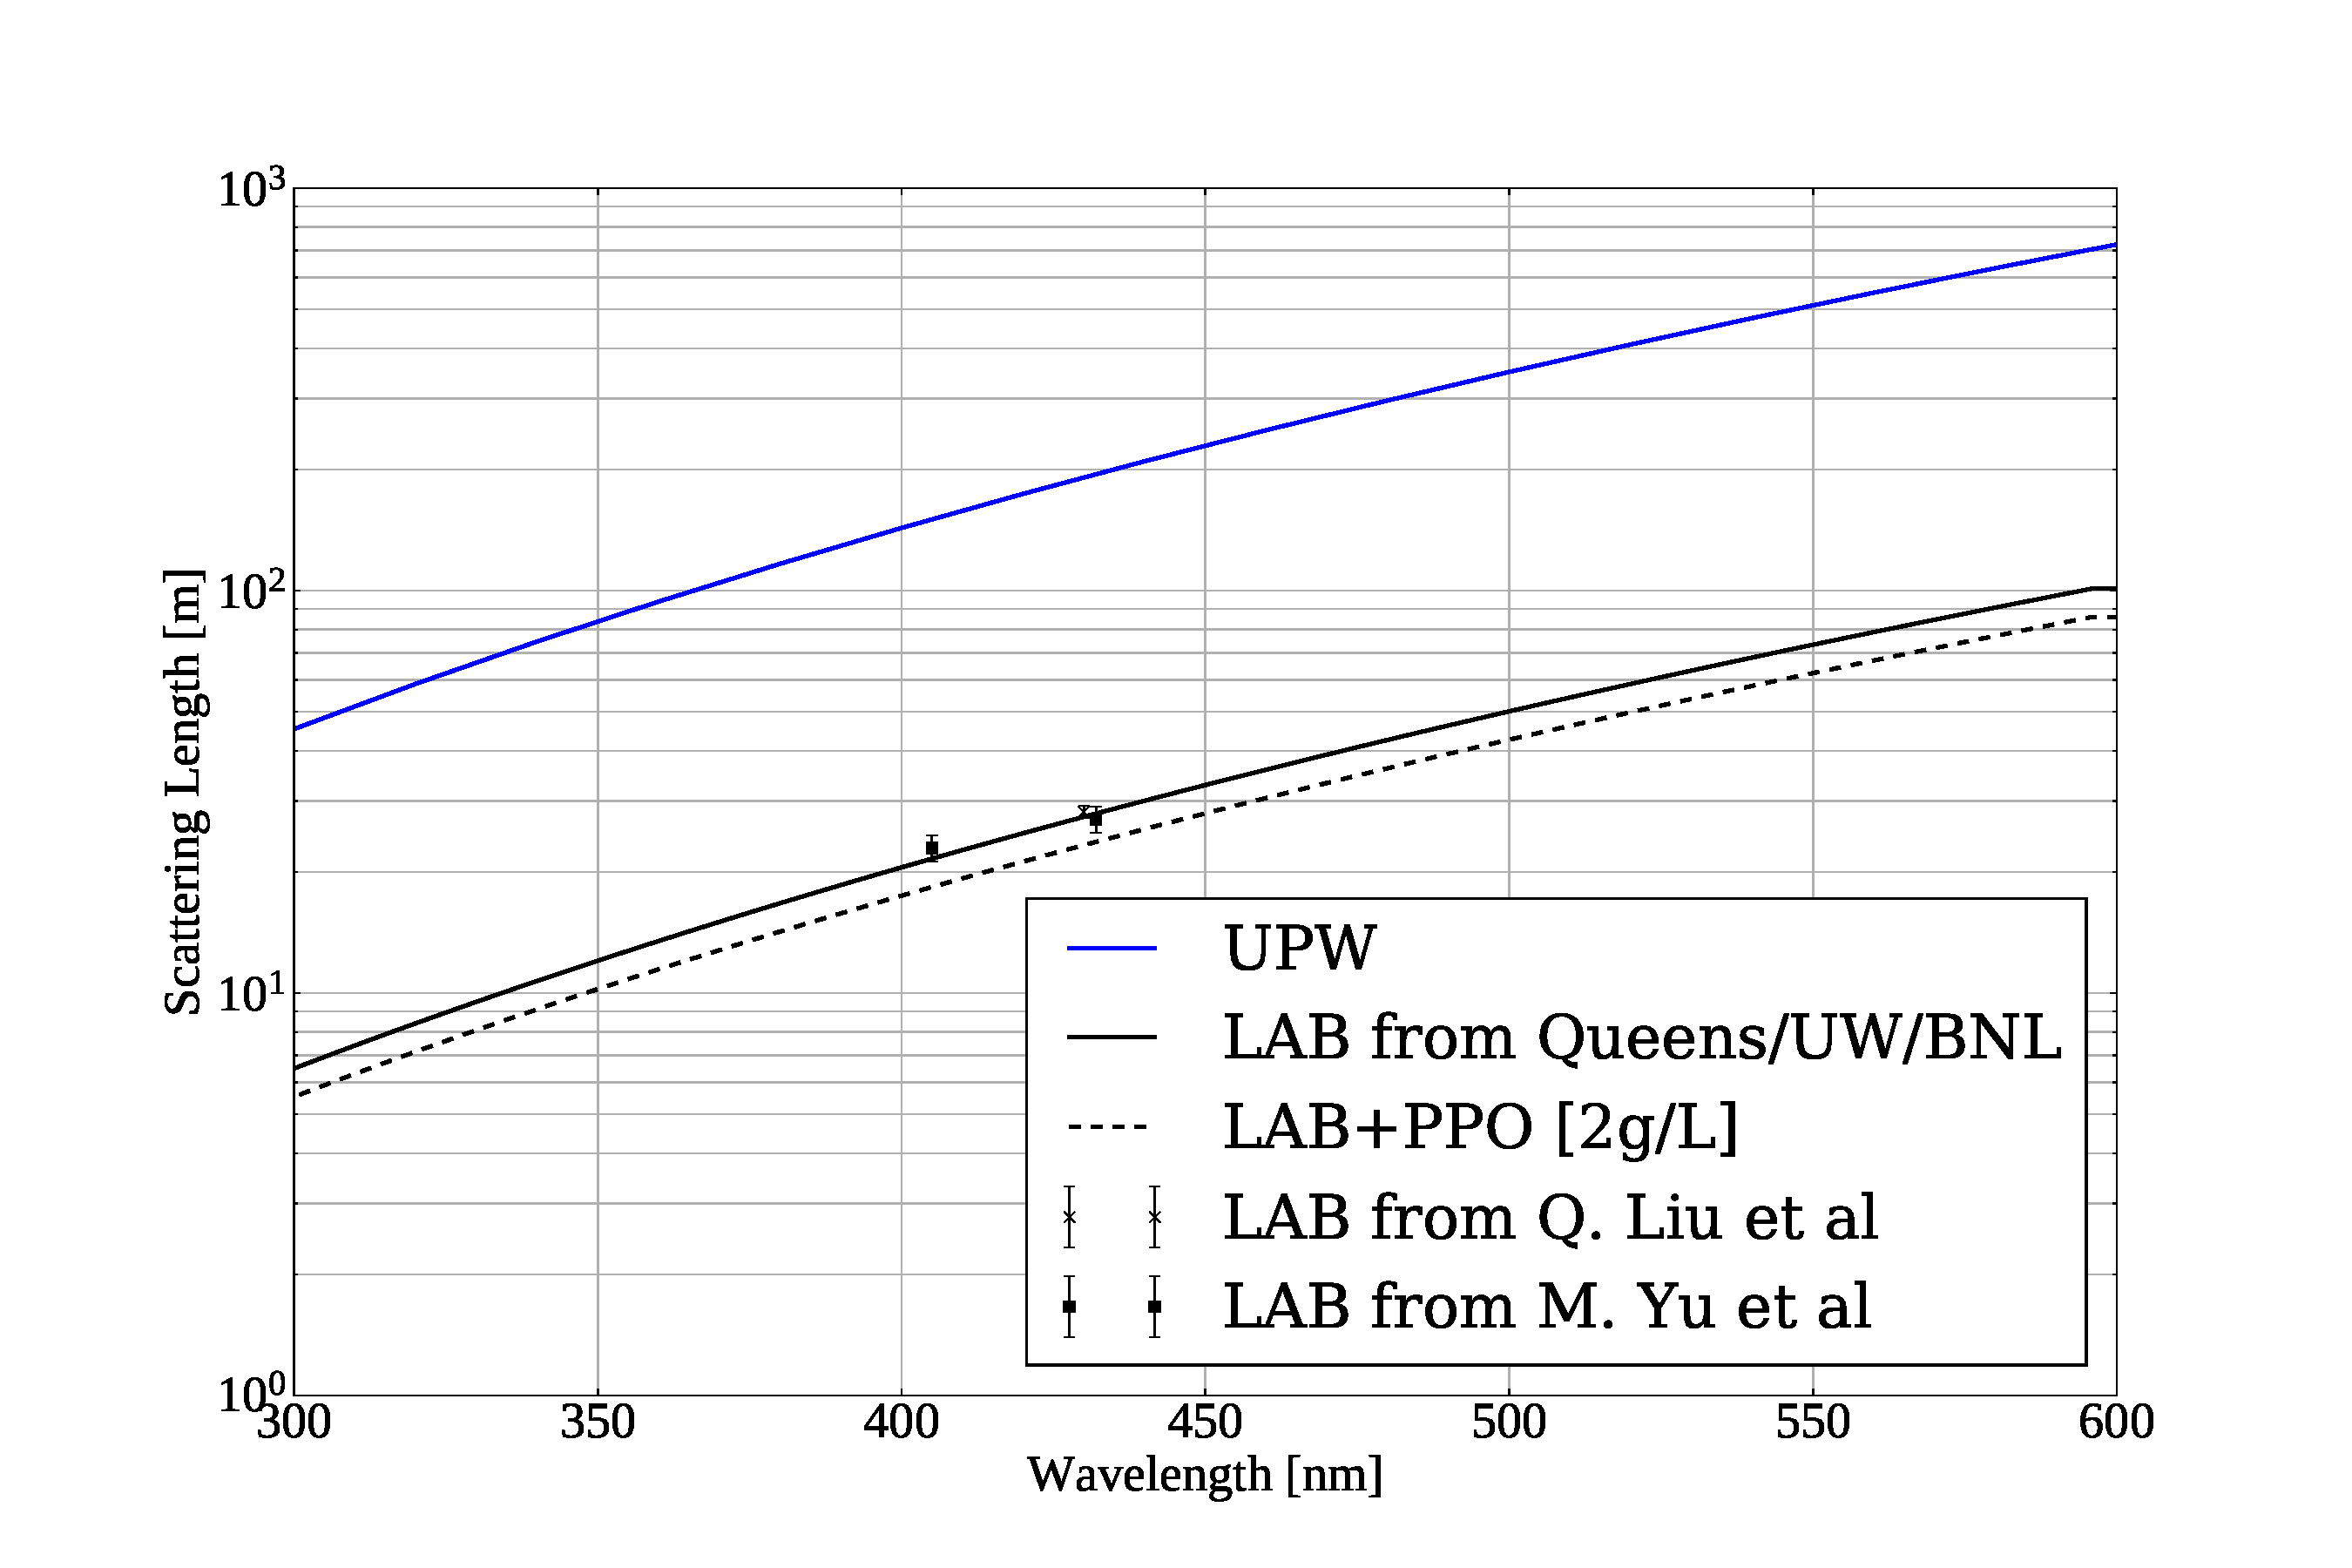
\includegraphics[width=0.8\linewidth]{2_Detector/Figs/scattering_lengths_plot.pdf}
    \caption[Scattering lengths in simulation for UPW, LAB, and \SI{2.2}{\gpl} LAB-PPO]
    {Scattering lengths used in simulation for UPW, LAB, and \SI{2}{\gpl} LAB-PPO. The UPW shape is taken from indirect in-situ measurements in~\cite{moffatOpticalCalibrationSudbury2001} with an additional divisive scaling factor from~\cite{turnerMeasurementScatteringCharacteristics2022}. The LAB shape is taken from ex-situ measurements by SNO+ members at Queen's University, University of Washington, and Brookhaven National Laboratory~\cite{chenOpticalPropertiesRAT2012,seguiScintillatorModelComparison2015}. An additional divisive scaling factor of 1.176 due to PPO was made by~\cite{liuAttenuationScatteringTeBD2016}. For comparison, measurements by members of the JUNO Collaboration for LAB are also shown~\cite{liuRayleighScatteringDepolarization2015,yuMeasurementsRayleighRatios2022}.}
    \label{fig:scattering_lengths_upw_labppo_current}
\end{figure}

    % \begin{itemize}
    %     \item Explain the electrodynamical model for scattering, giving rise to the expected $1/\lambda^4$ wavelength-dependence of the scattering length, as well as the $1+\cos^2\theta$ dependence of the scattering angle.
    %     \item Describe how the density-fluctuation theory gives rise to a possible modification to the scattering angle distribution due to the anisotropy of the optical media's polarisability vector. Studies by JUNO have shown that LAB-PPO has such a measurable anisotropy.
    %     \item Show the existing model for water and LAB-PPO used in RAT, and note that this anisotropy is currently not included in any simulations. I don't need to go in too much detail for this subsection as Krish did a nice job in his thesis and I can cite that, but I do need to write enough to cover the basics for my SMELLIE analysis chapter.
    % \end{itemize}
    % [3 pages]

\subsubsection{Absorption and Re-emission}
In addition to scattering, an optical medium is also able to absorb light that propagates through it. For a given medium, the \textit{absorption length} $l_{\mathrm{abs}}$ is analogous to $l_{\mathrm{Ray}}$ described above, and is typically strongly a function of wavelength. For most materials, absorbed light is forever lost, converted into heat. However, for the special case of scintillators, re-emission of absorbed light is possible: this is because of the physics described in Section~\ref{sec:scintillation}.

Because both scattering and absorption impede a photon's ability to propagate through a medium directly, it is often possible to measure their combined impact through what is known as the attenuation/extinction length, $l_{\mathrm{ext}}$:
\begin{equation}\label{eq:ext_length_def}
    \frac{1}{l_{\mathrm{ext}}} = \frac{1}{l_{\mathrm{abs}}} + \frac{1}{l_{\mathrm{Ray}}}.
\end{equation}
In the water phase, the `Laserball' calibration system was used by Ana Sofia In\'{a}cio to measure various optical properties of the detector, including the extinction lengths of the UPW and acrylic as a function of wavelength~\cite{andersonOpticalCalibrationSNO2021,inacioDataAnalysisWater2022}. Using the water phase scattering measurements made by E. Turner, Eq.~\ref{eq:ext_length_def} allowed for the estimation of the absorption lengths of these two materials, shown in Figure~\ref{fig:abs_lengths_optics_paper}. Measurements of the extinction length in the scintillator phase is discussed in detail in Chapter~\ref{chap:smellie_analysis}.

\begin{figure}
    \centering
    \begin{subfigure}{0.98\textwidth}
        \centering
        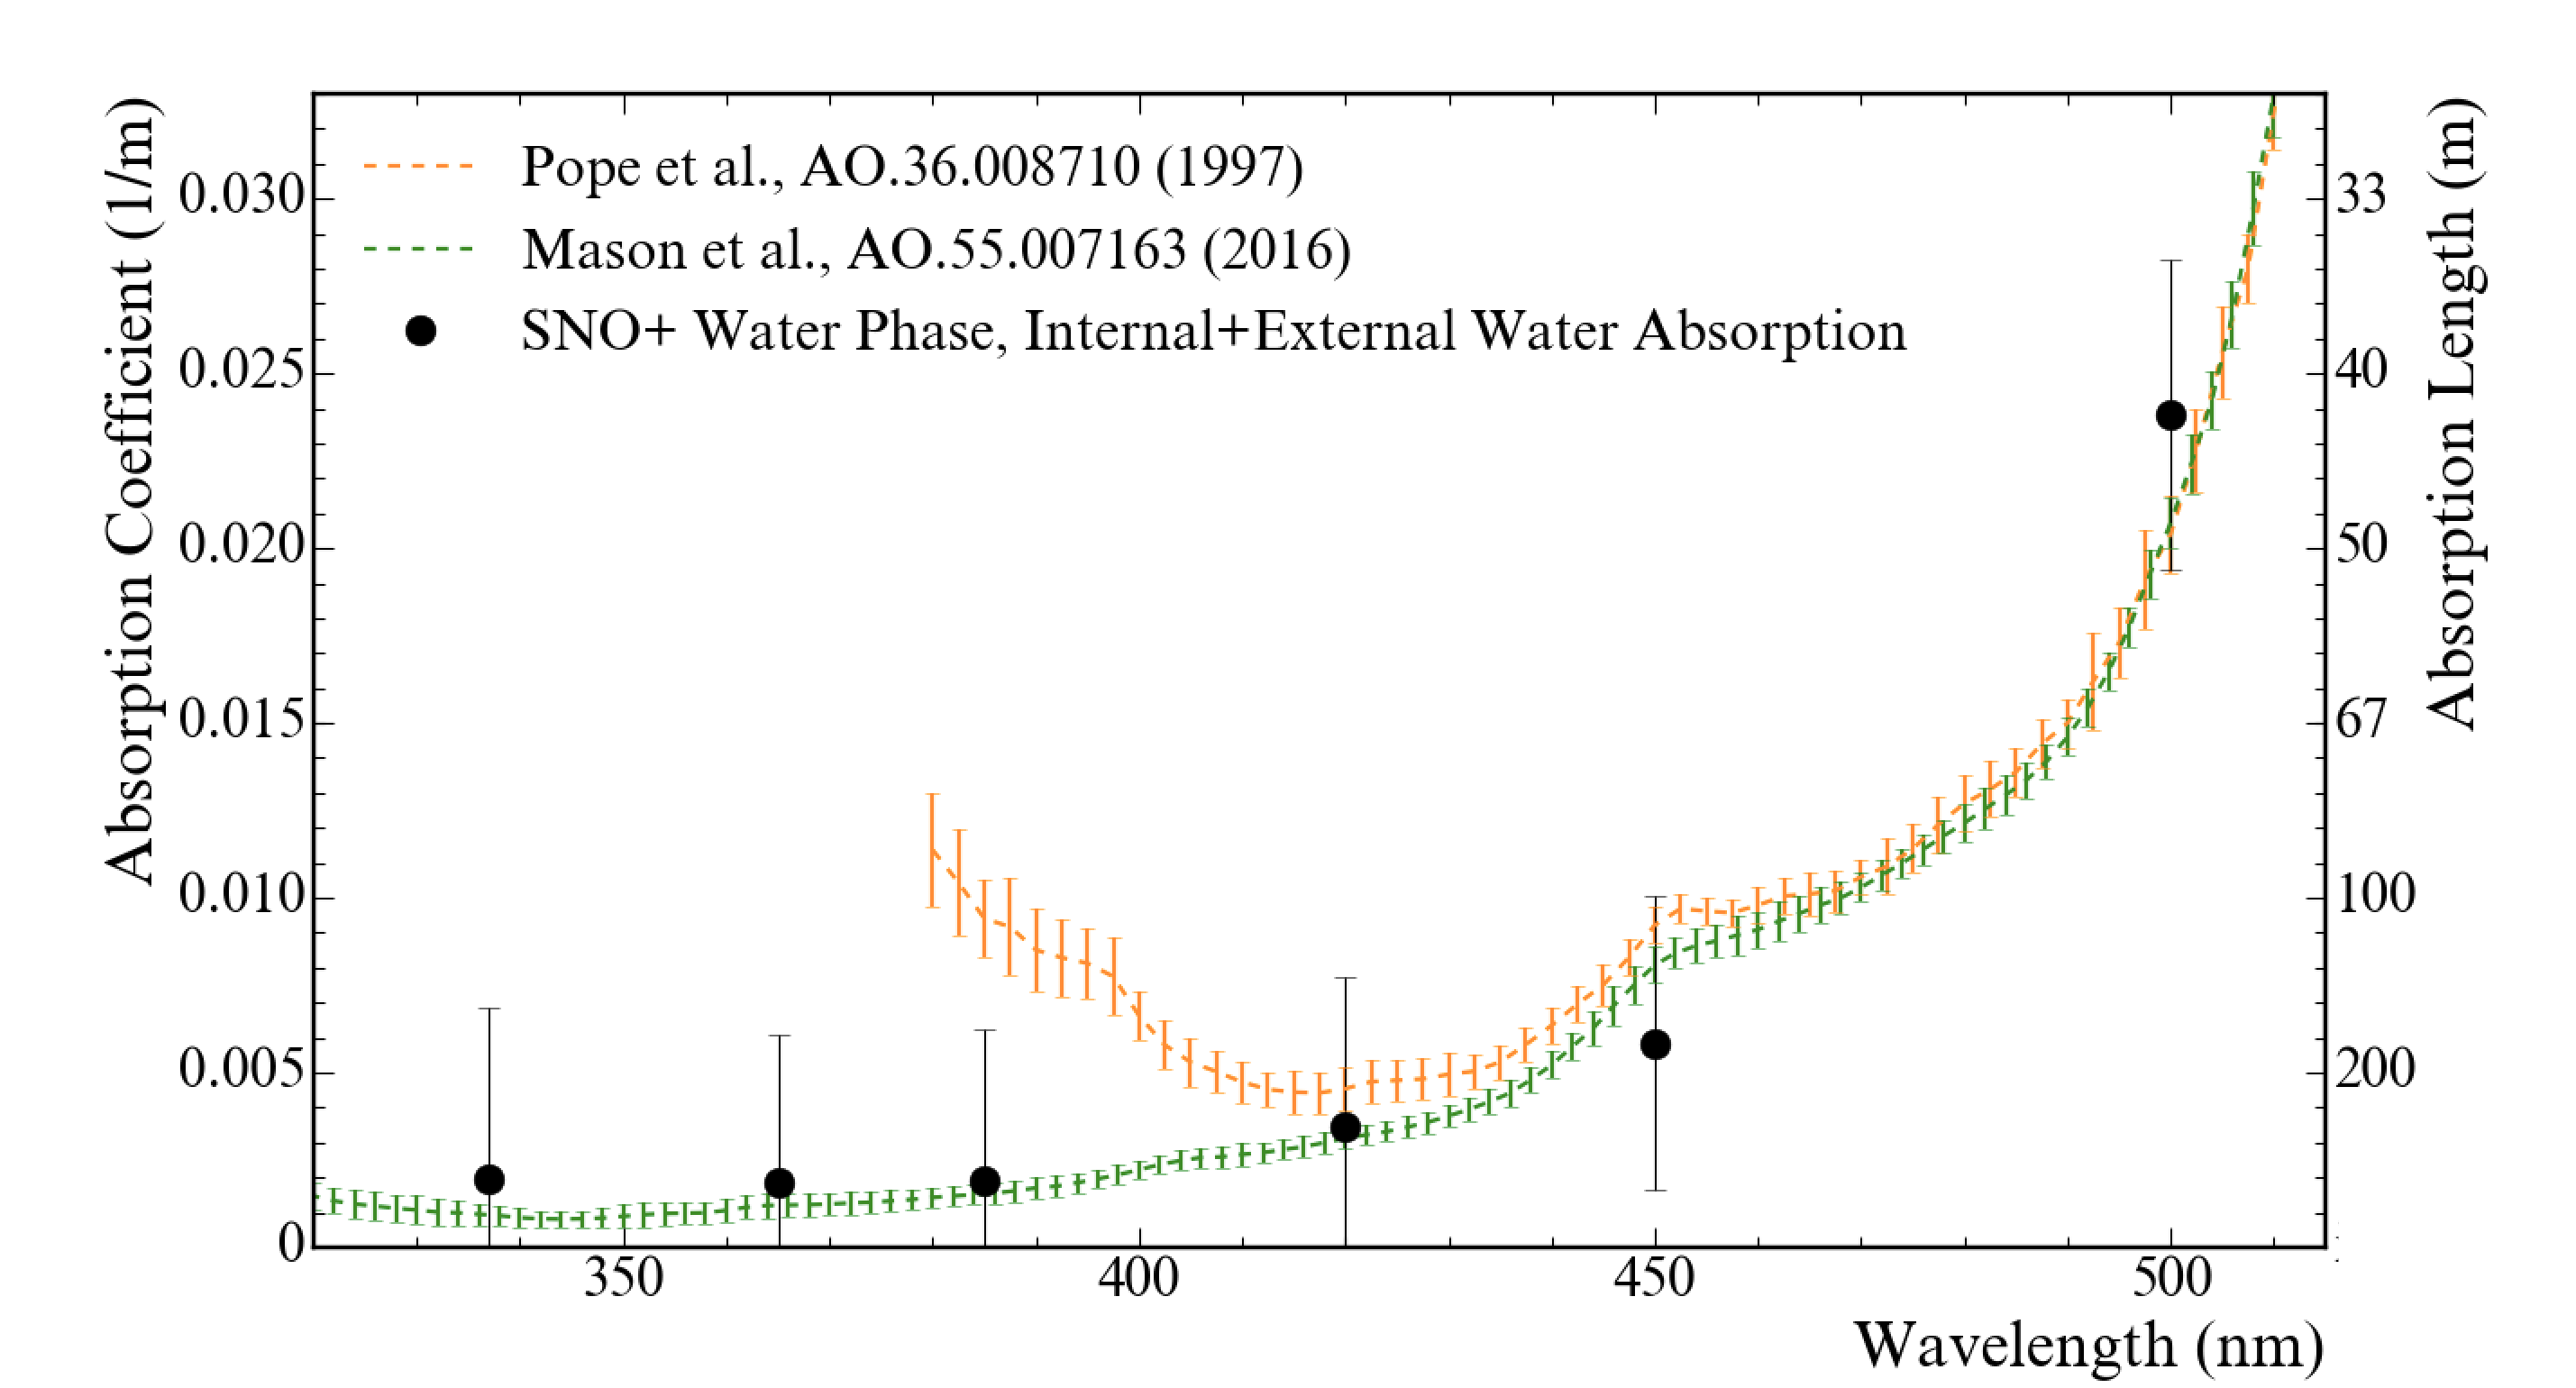
\includegraphics[width=0.9\textwidth]{2_Detector/Figs/WaterAbsorption.png}
        \caption{UPW optical absorption}
        \label{fig:abs_length_water_optics_paper}
    \end{subfigure}
    \begin{subfigure}{0.98\textwidth}
        \centering
        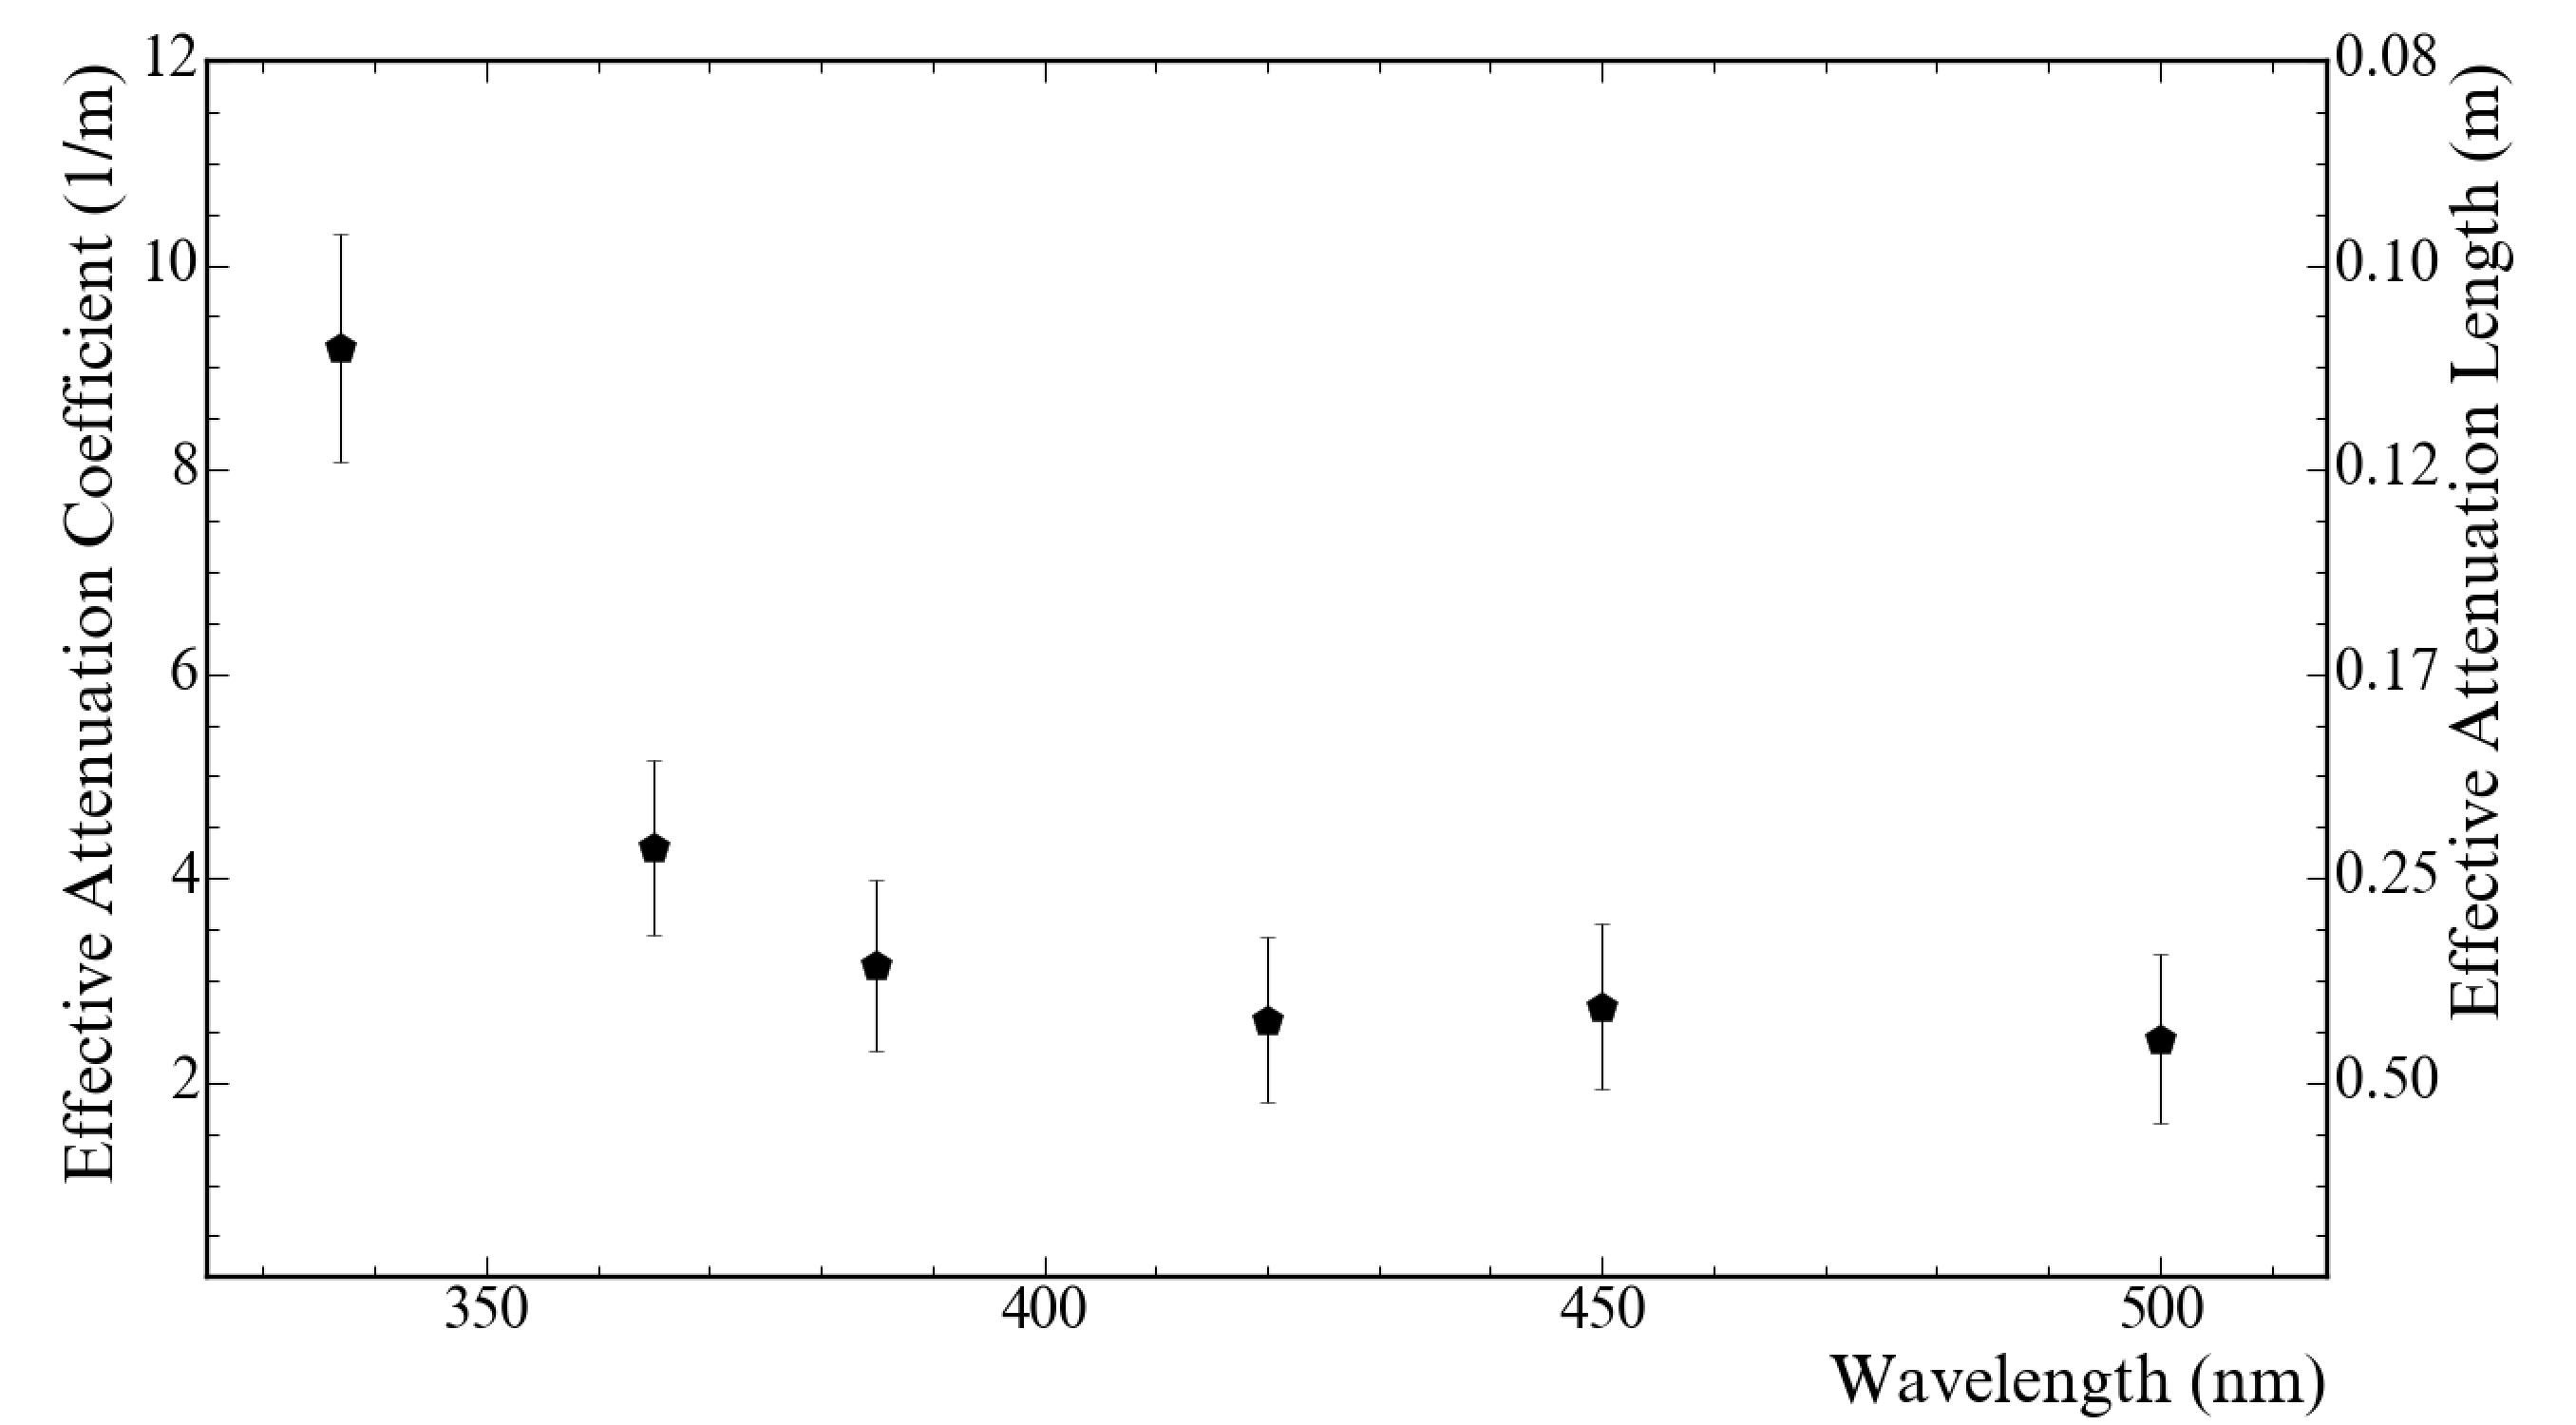
\includegraphics[width=0.85\textwidth]{2_Detector/Figs/AcrylicAttenuation.png}
        \caption{Acrylic optical attenuation}
        \label{fig:abs_length_acylic_optics_paper}
    \end{subfigure}
    \caption[Measured properties of the UPW and acrylic in the water phase.]
    {Properties of the UPW and acrylic in the water phase, measured by A. S. In\'{a}cio in~\cite{andersonOpticalCalibrationSNO2021,inacioDataAnalysisWater2022}.}
    \label{fig:abs_lengths_optics_paper}
\end{figure}

    % \begin{itemize}
    %     \item State that light can get absorbed by materials, and if that medium is a scintillator then re-emission is possible. I think further details such as the specific shape of the absorption/re-emission of the scintillator and water can be shown in the SMELLIE analysis chapter, in which I have to explain about possible changes to the model anyway.
    % \end{itemize}
    % [1/2 page]
\subsubsection{Surface reflection and refraction}
\nomenclature{\textbf{TIR}}{Total Internal Reflection}
When light travels through the boundary between media, both reflection and refraction can be possible, depending on the relative refractive indices of the two media as well as the angle of incidence. The refractive indices of the UPW, acrylic, and LAB-PPO are shown as a function of wavelength in Figure~\ref{fig:ref_indices_snoplus}. Note that, for most optical wavelengths, LAB-PPO has a very close refractive index to acrylic, whereas UPW is somewhat farther away. By consequence, negligible refraction is expected in most cases for light travelling between the liquid scintillator and the acrylic; however, substantial refraction and reflection are possible for light travelling between acrylic and UPW. Because of this, isotropically-emitting point-like physics events within the AV that are close enough to the acrylic will have some of their light undergo Total Internal Reflection (TIR) at the AV, reflecting back into the AV instead of continuing outward into the outer water.

% \begin{figure}
%     \centering
%     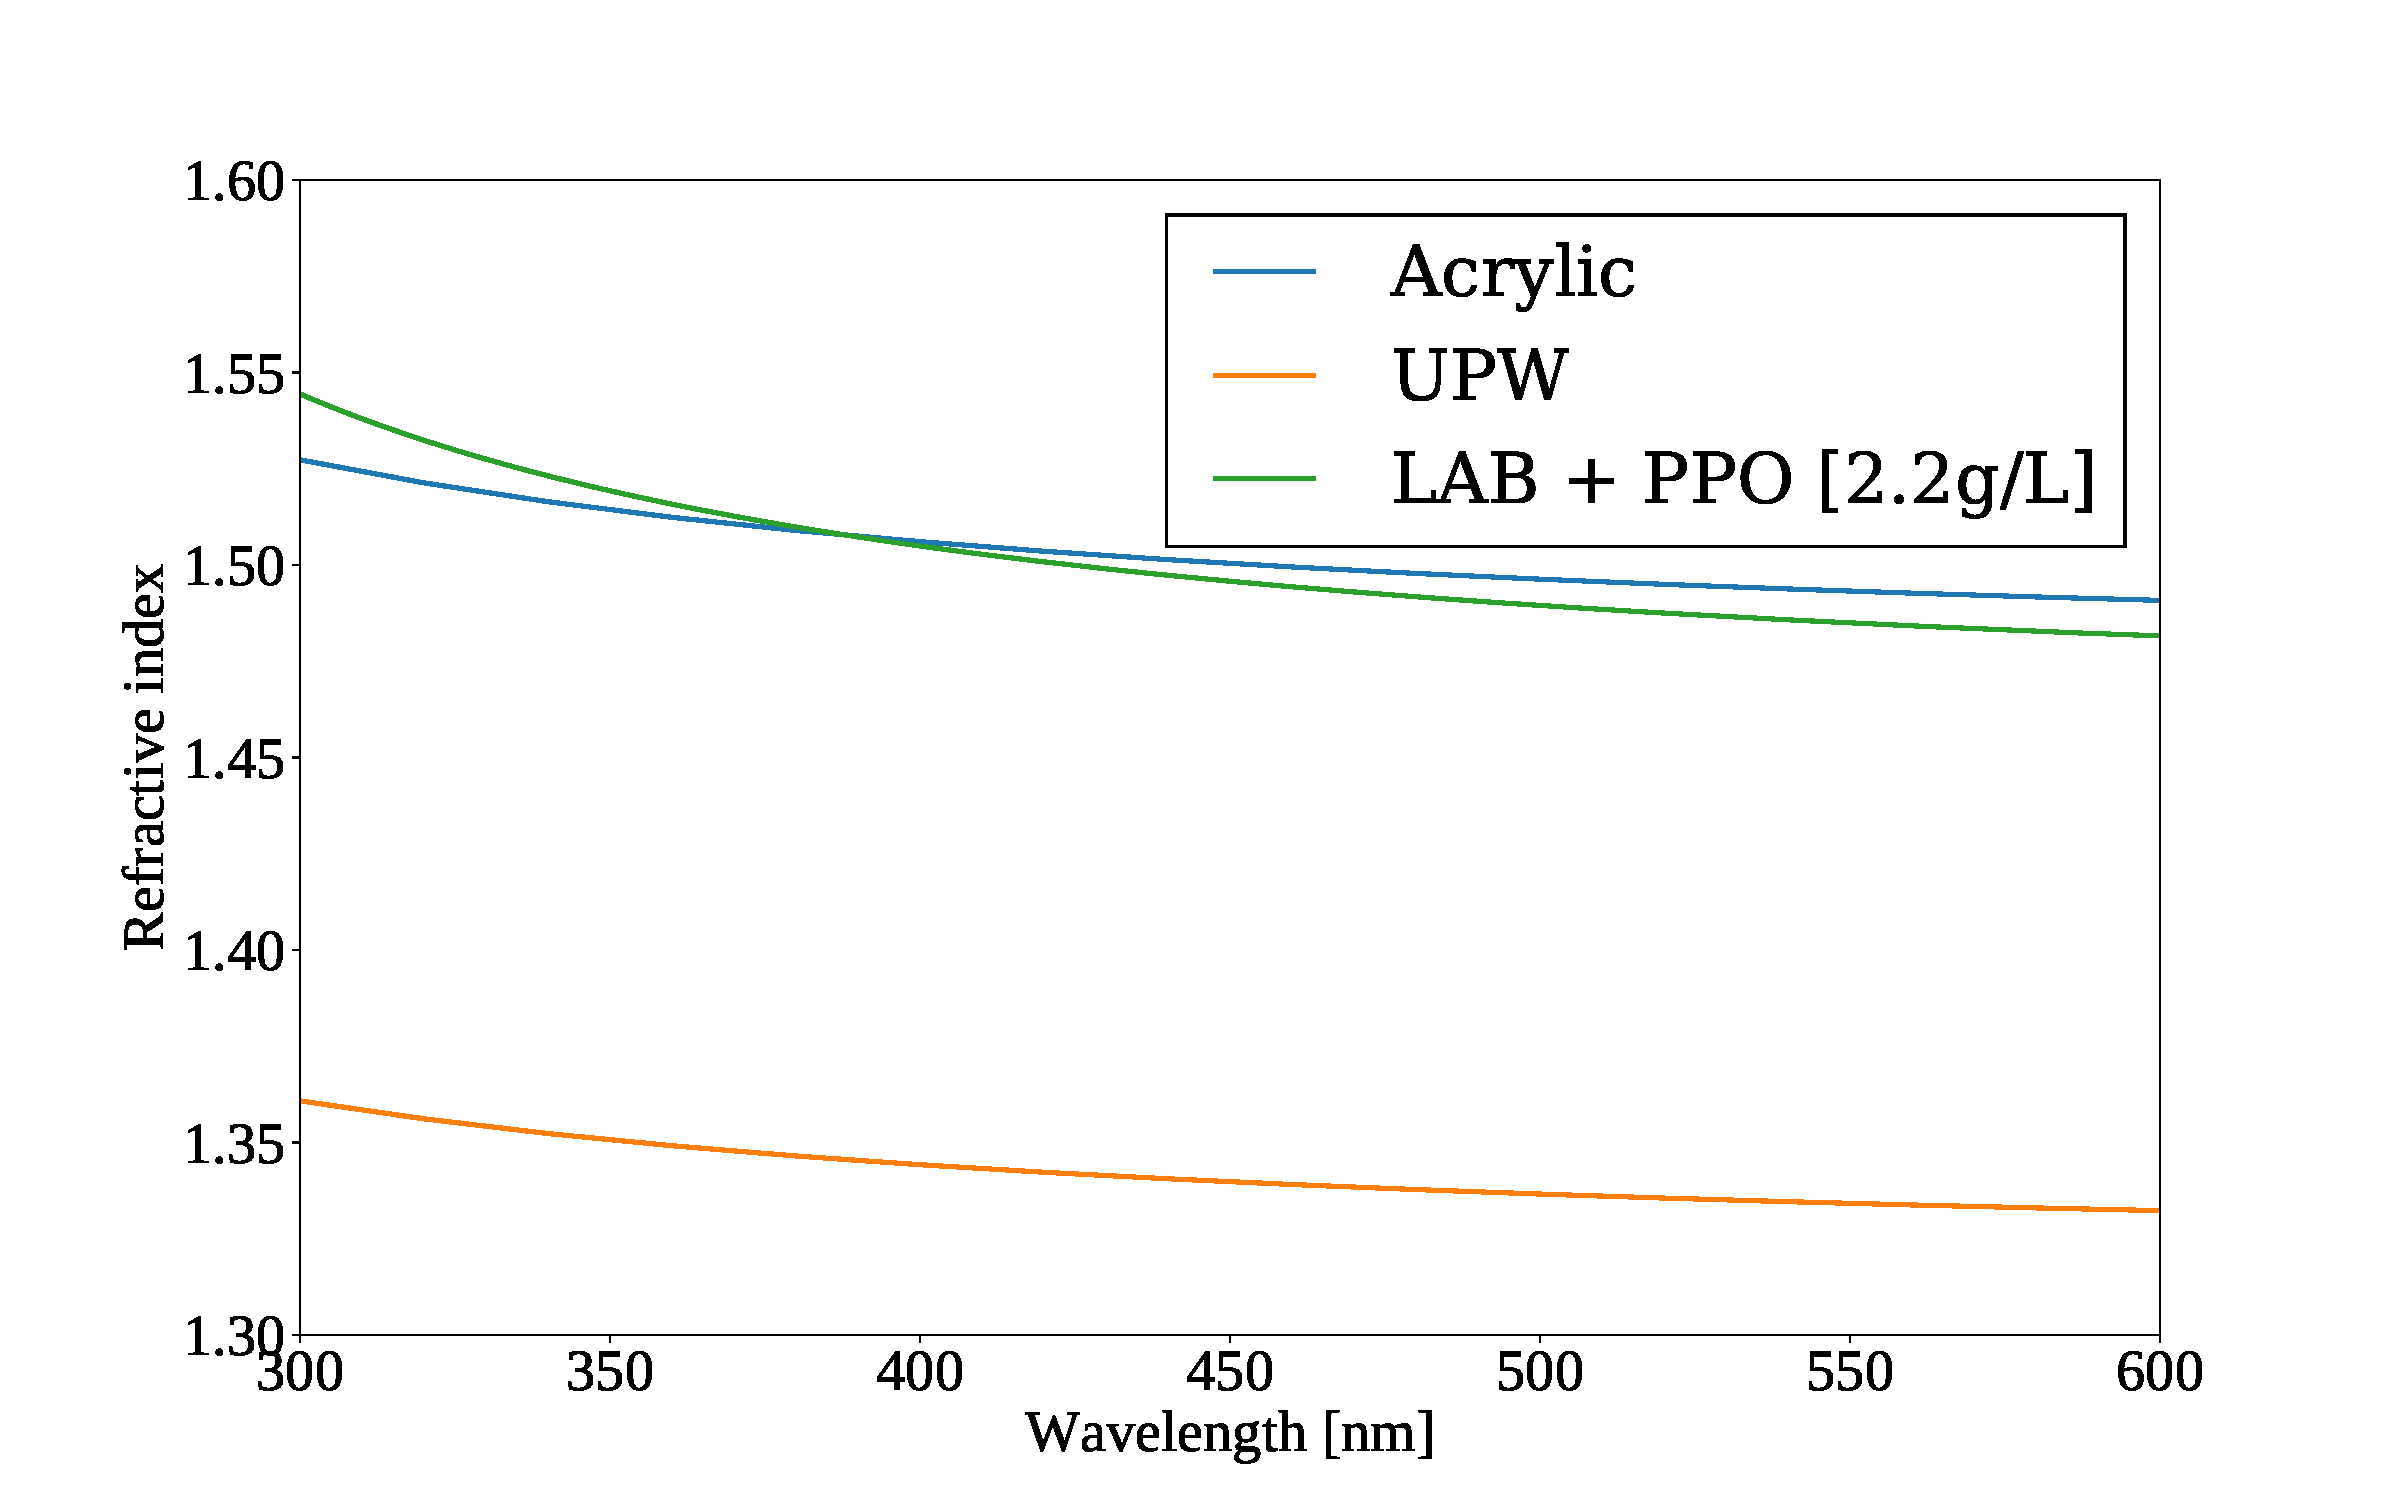
\includegraphics[width=0.8\linewidth]{2_Detector/Figs/refractive_indices_plot.pdf}
%     \caption[Refractive indices of acrylic, UPW, and LAB-PPO as a function of wavelength]
%     {Refractive indices of acrylic, UPW, and LAB-PPO as a function of wavelength~\cite{andersonOpticalCalibrationSNO2021,tseungEllipsometricMeasurementsRefractive2011,moffatOpticalCalibrationSudbury2001}. % cite!
%     }
%     \label{fig:ref_indices_snoplus}
% \end{figure}

\begin{figure}
    \centering
    \begin{subfigure}{0.48\textwidth}
        \centering
        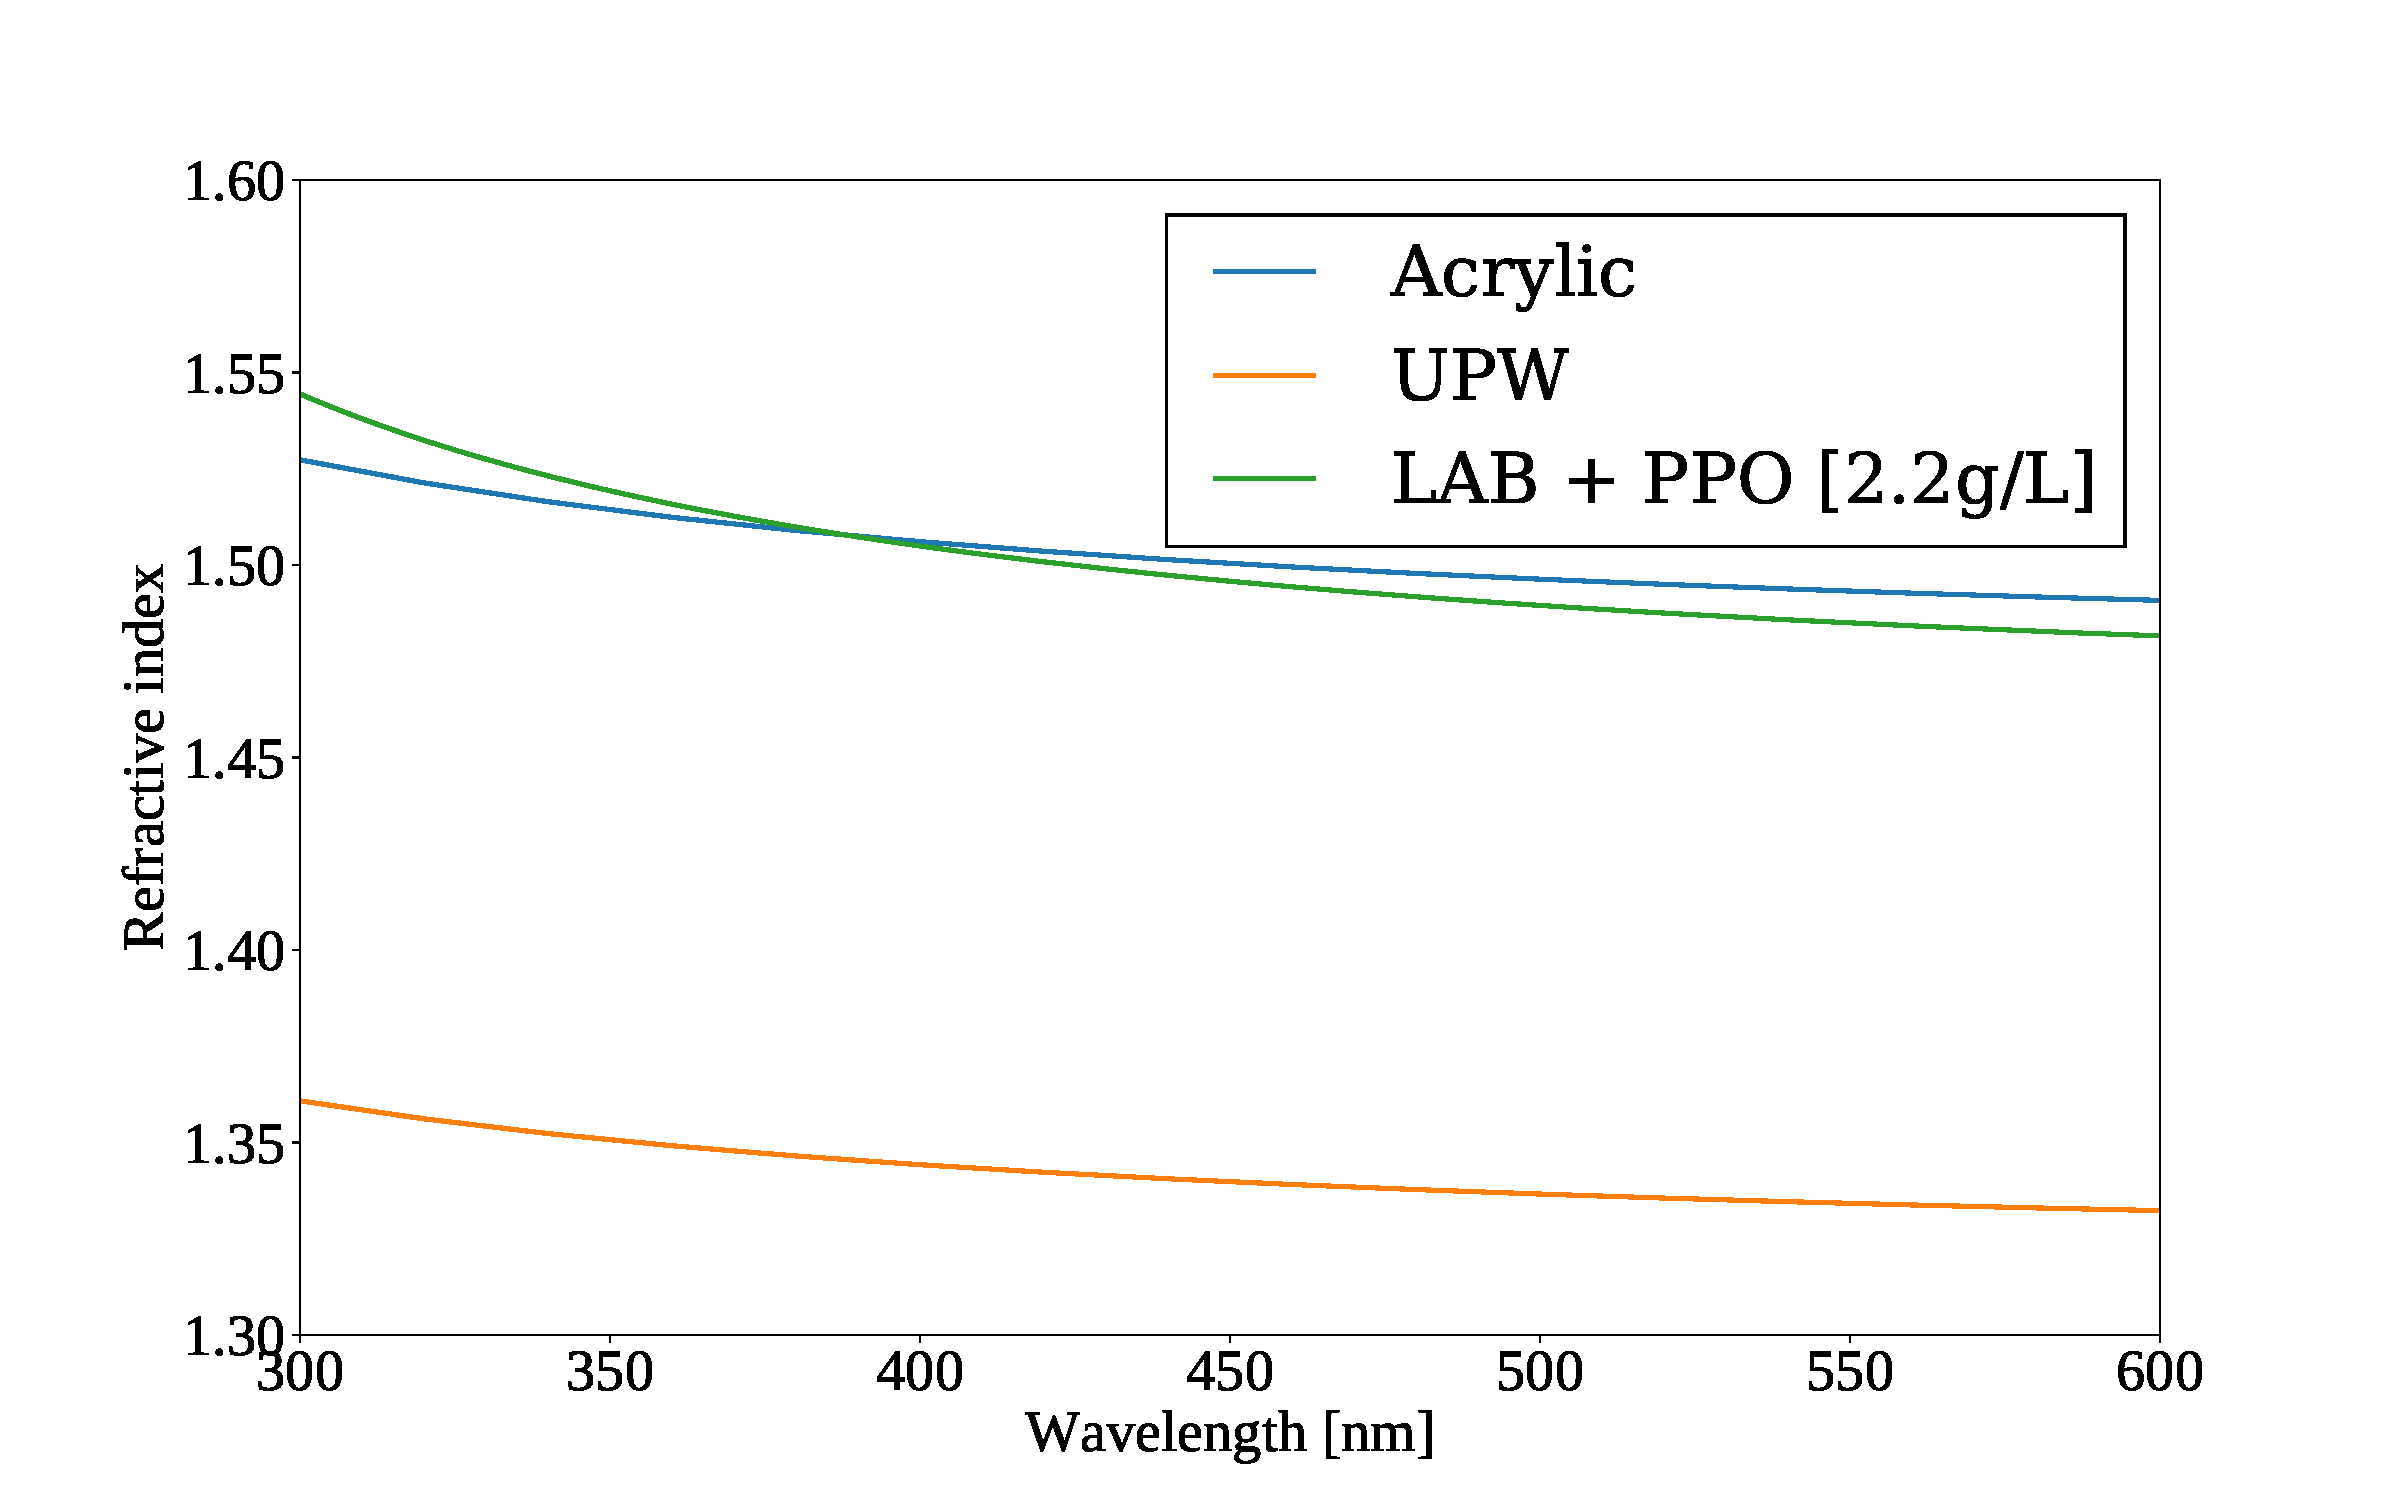
\includegraphics[width=0.95\linewidth]{2_Detector/Figs/refractive_indices_plot.pdf}
        \caption{}
        \label{fig:ref_indices_snoplus}
    \end{subfigure}
    \begin{subfigure}{0.48\textwidth}
        \centering
        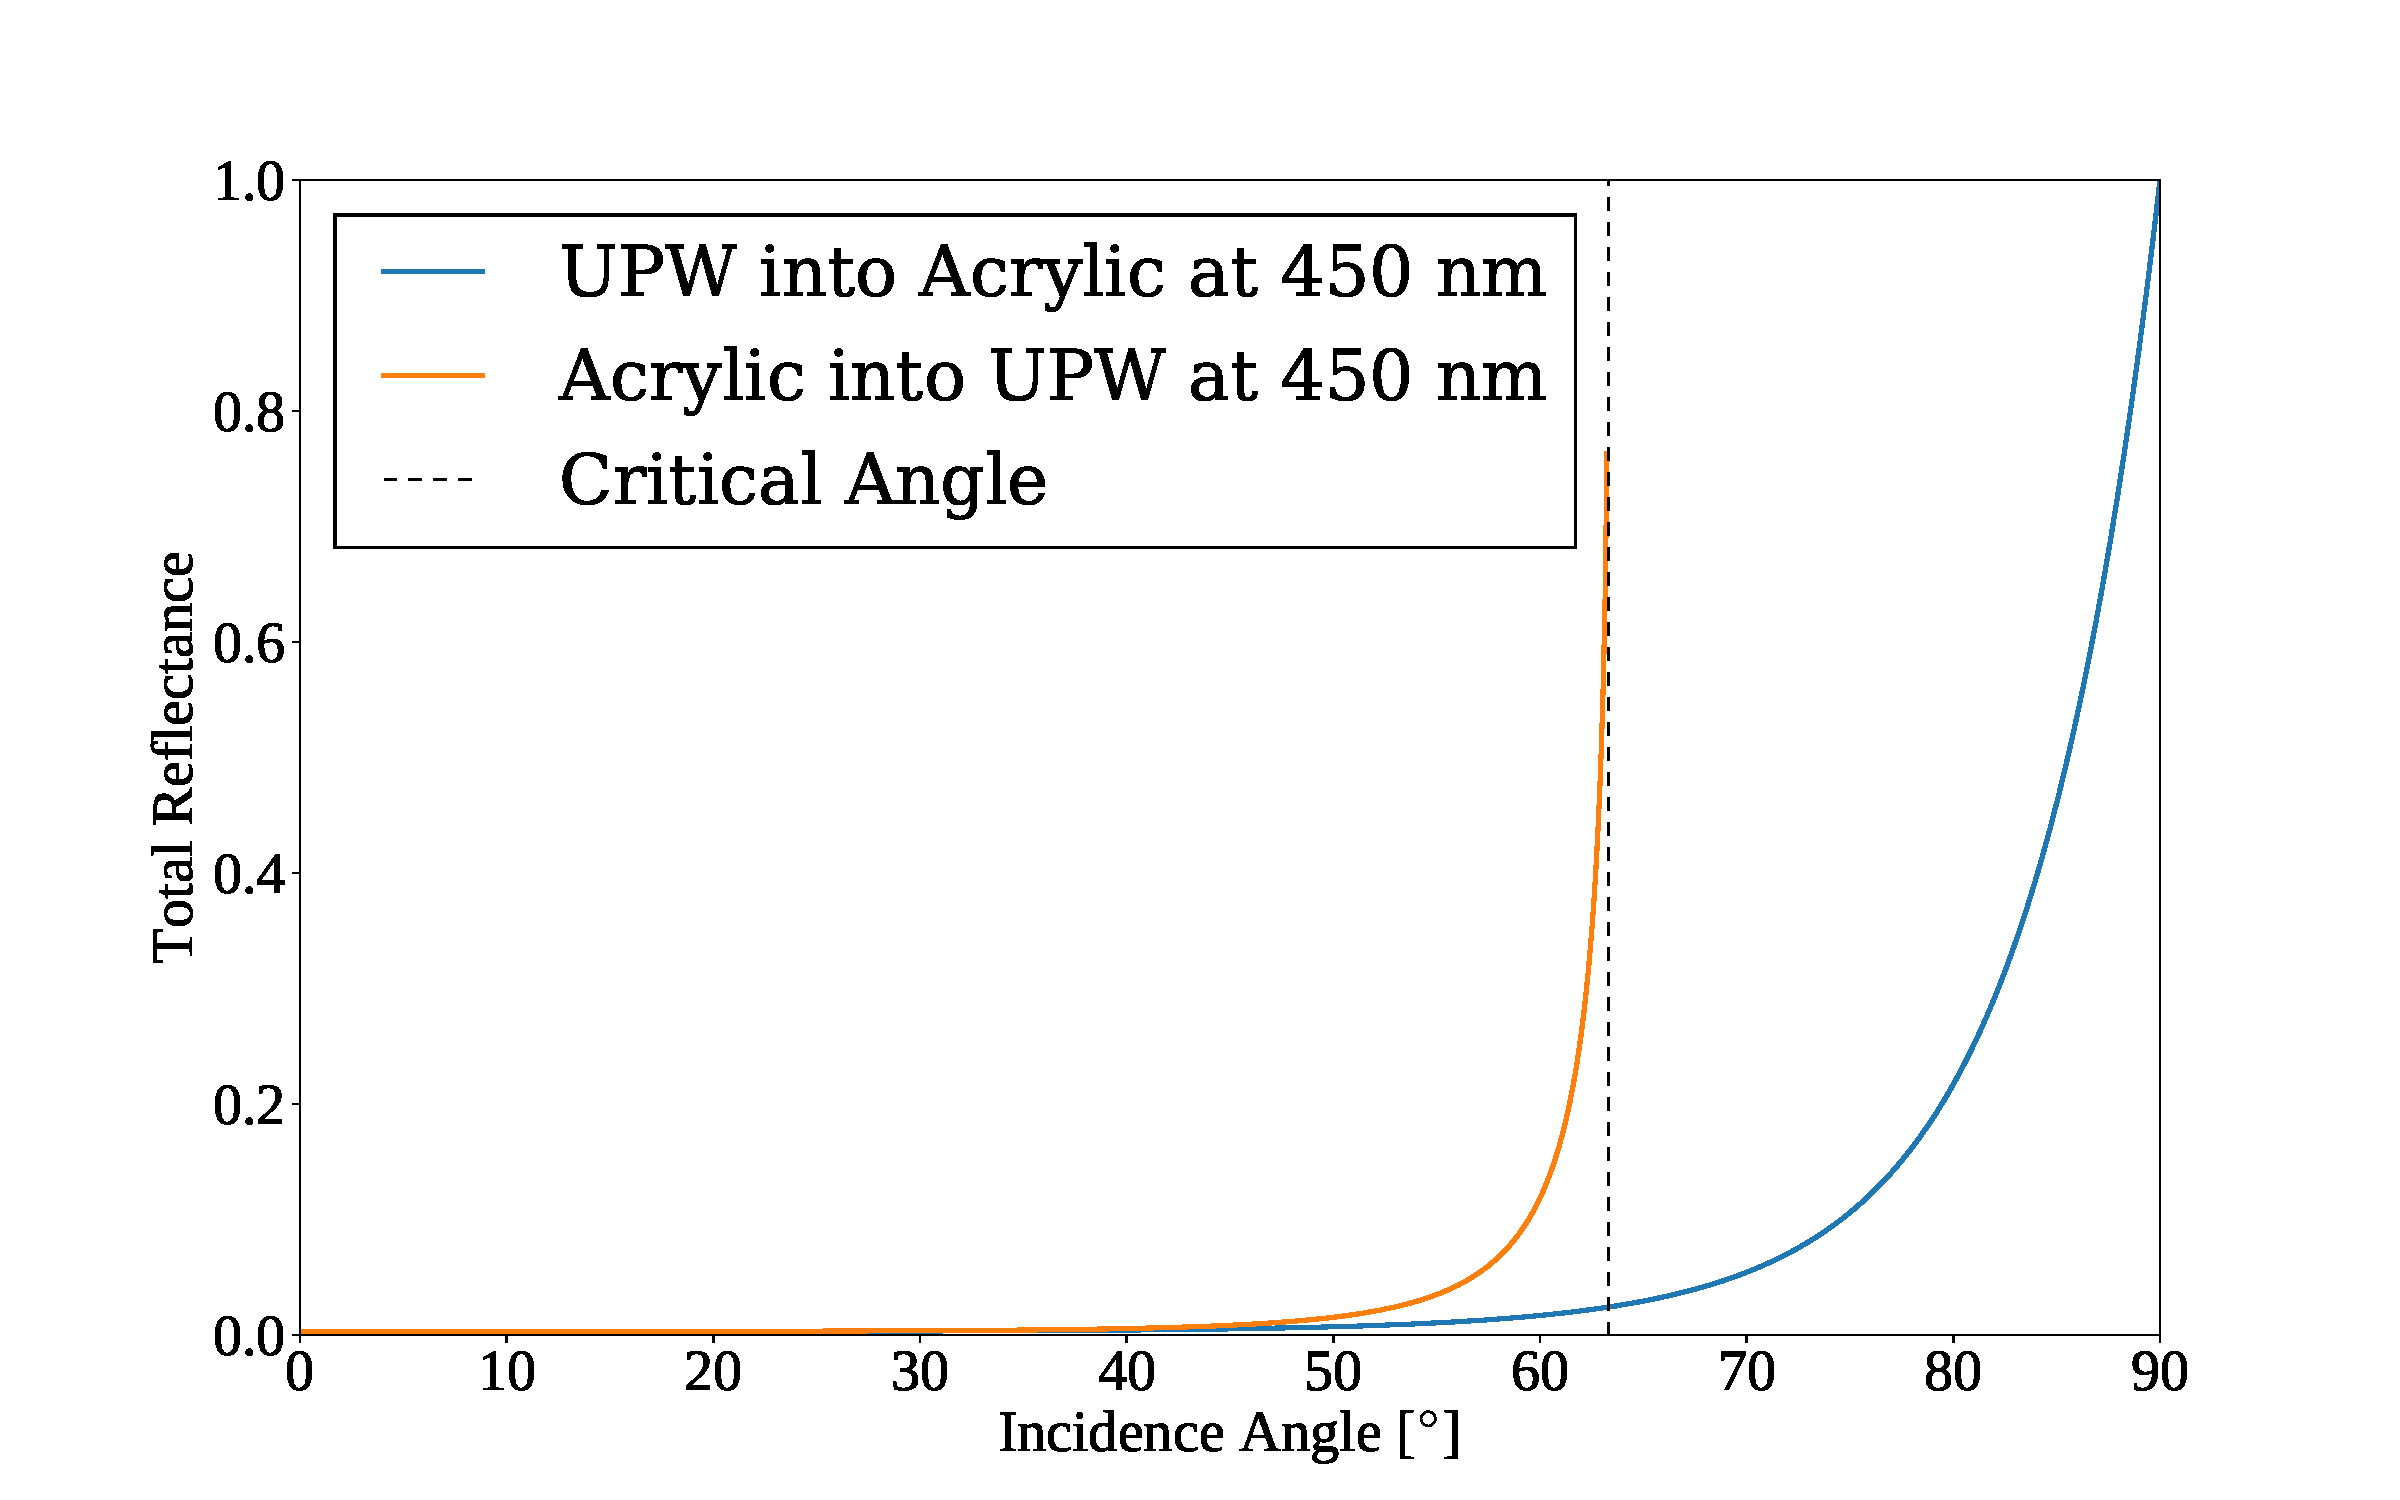
\includegraphics[width=0.95\linewidth]{2_Detector/Figs/reflectance_vs_angle_plot.pdf}
        \caption{}
        \label{fig:reflectance_vs_angle}
    \end{subfigure}
    \caption[Refractive indices of acrylic, UPW, and LAB-PPO as a function of wavelength; also reflectance as a function of incidence angle]
    {\textbf{(a):} Refractive indices of acrylic, UPW, and LAB-PPO as a function of wavelength. The values for acrylic and UPW come from model fits to data made in SNO~\cite{boardmanDetectionCherenkovRadiation1992,moffatOpticalCalibrationSudbury2001}, whereas those for LAB-PPO come from data taken in~\cite{tseungEllipsometricMeasurementsRefractive2011}. \textbf{(b):} Reflectance of an unpolarised beam of light at \SI{450}{\nm} going between UPW and acrylic.
    }
    \label{fig:ref_index_and_reflectance}
\end{figure}

Even when not undergoing TIR, some light at a boundary will still reflect. The fraction of light that reflects is known as the \textit{reflectance} $R$, compared to that which is able to transmit through the boundary, the \textit{transmittance} $T=1-R$. The \textit{Fresnel Equations} determine the reflectance of an interface~\cite{hechtSectionFresnelEquations2014}:% Fresnel eqs: Hecht?
\begin{equation}
    R_{s} = \left|\frac{n_{1}\cos{\theta_{i}}-n_{2}\cos{\theta_{t}}}{n_{1}\cos{\theta_{i}}+n_{2}\cos{\theta_{t}}}\right|^{2},\\
    R_{p} = \left|\frac{n_{1}\cos{\theta_{t}}-n_{2}\cos{\theta_{i}}}{n_{1}\cos{\theta_{t}}+n_{2}\cos{\theta_{i}}}\right|^{2},
\end{equation}
where $R_{s}$ and $R_{p}$ are the reflectances of $s$- and $p$-polarised light, $n_{1}$ and $n_{2}$ are the refractive indices of the first and second optical media, and $\theta_{i}$ and $\theta_{t}$ are the angles of incidence and refraction, respectively. In SNO+, there is no sensitivity of the PMTs to different polarisations, so what matters is the total reflectance $R = \left(R_{s}+R_{p}\right)/2$.

The total reflectance going from UPW into acrylic, as well as from acrylic into UPW, for an unpolarised beam of light with wavelength \SI{450}{\nm} is shown in Fig.~\ref{fig:reflectance_vs_angle}. For the latter case, the critical angle at which TIR occurs is clear.

    % \begin{itemize}
    %     \item State that boundaries between media can induce reflections and refraction, as governed by the Fresnel transmission and reflection formulae. These formulae are worth mentioning because I use them in my SMELLIE extinction length analysis.
    % \end{itemize}
    % [1/2 page]
\subsection{Detection by PMTs}\label{sec:pmts}
The final step for photons in the detector is detection by a PMT. Almost all PMTs in SNO+ are of the Hamamatsu R1408 design~\cite{BOGER2000172}. % cite
The PMTs within SNO+ are housed within an 18-segment reflecting Winston cone known as a `concentrator'. The combined PMT--concentrator `bucket', shown in Fig.~\ref{fig:pmt_conc_diagram}, is designed to maximise the collection efficiency of light emanating from within the AV, whilst minimising the collection efficiency of light outside the AV~\cite{moorheadReflectorsCherenkovDetectors1992}. % cite Moorhead
The so-called `angular response' of the PMT buckets has been measured in both SNO and SNO+ using the Laserball, which describes the relative collection efficiency as a function of the polar angle of the incident light ray relative to the direction in which the PMT bucket points. The results of this can be seen in Fig.~\ref{fig:pmt_angular_response}.

\begin{figure}
    \centering
    \begin{subfigure}{0.3\textwidth}
        \centering
        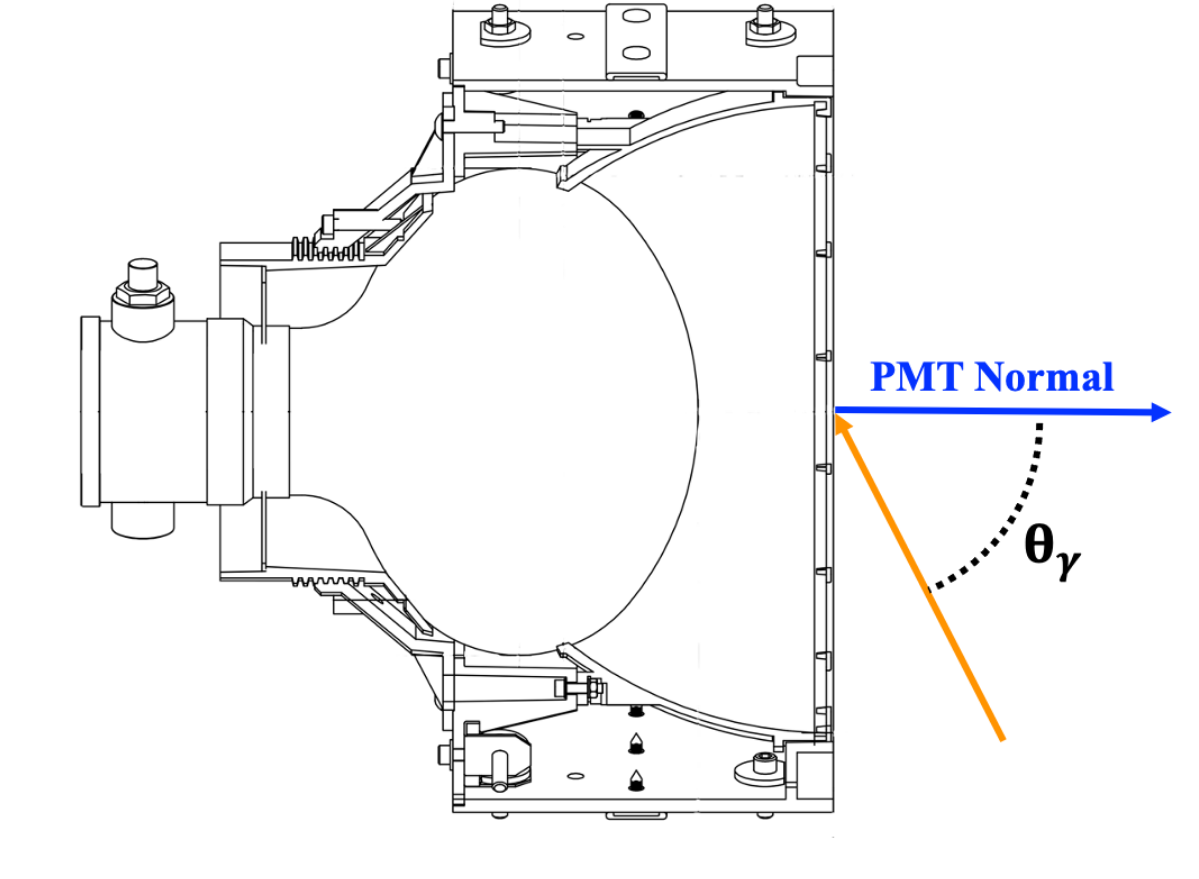
\includegraphics[width=0.95\textwidth]{2_Detector/Figs/pmt_bucket_assembly.png}
        \caption{}
        \label{fig:pmt_conc_diagram}
    \end{subfigure}
    \begin{subfigure}{0.69\textwidth}
        \centering
        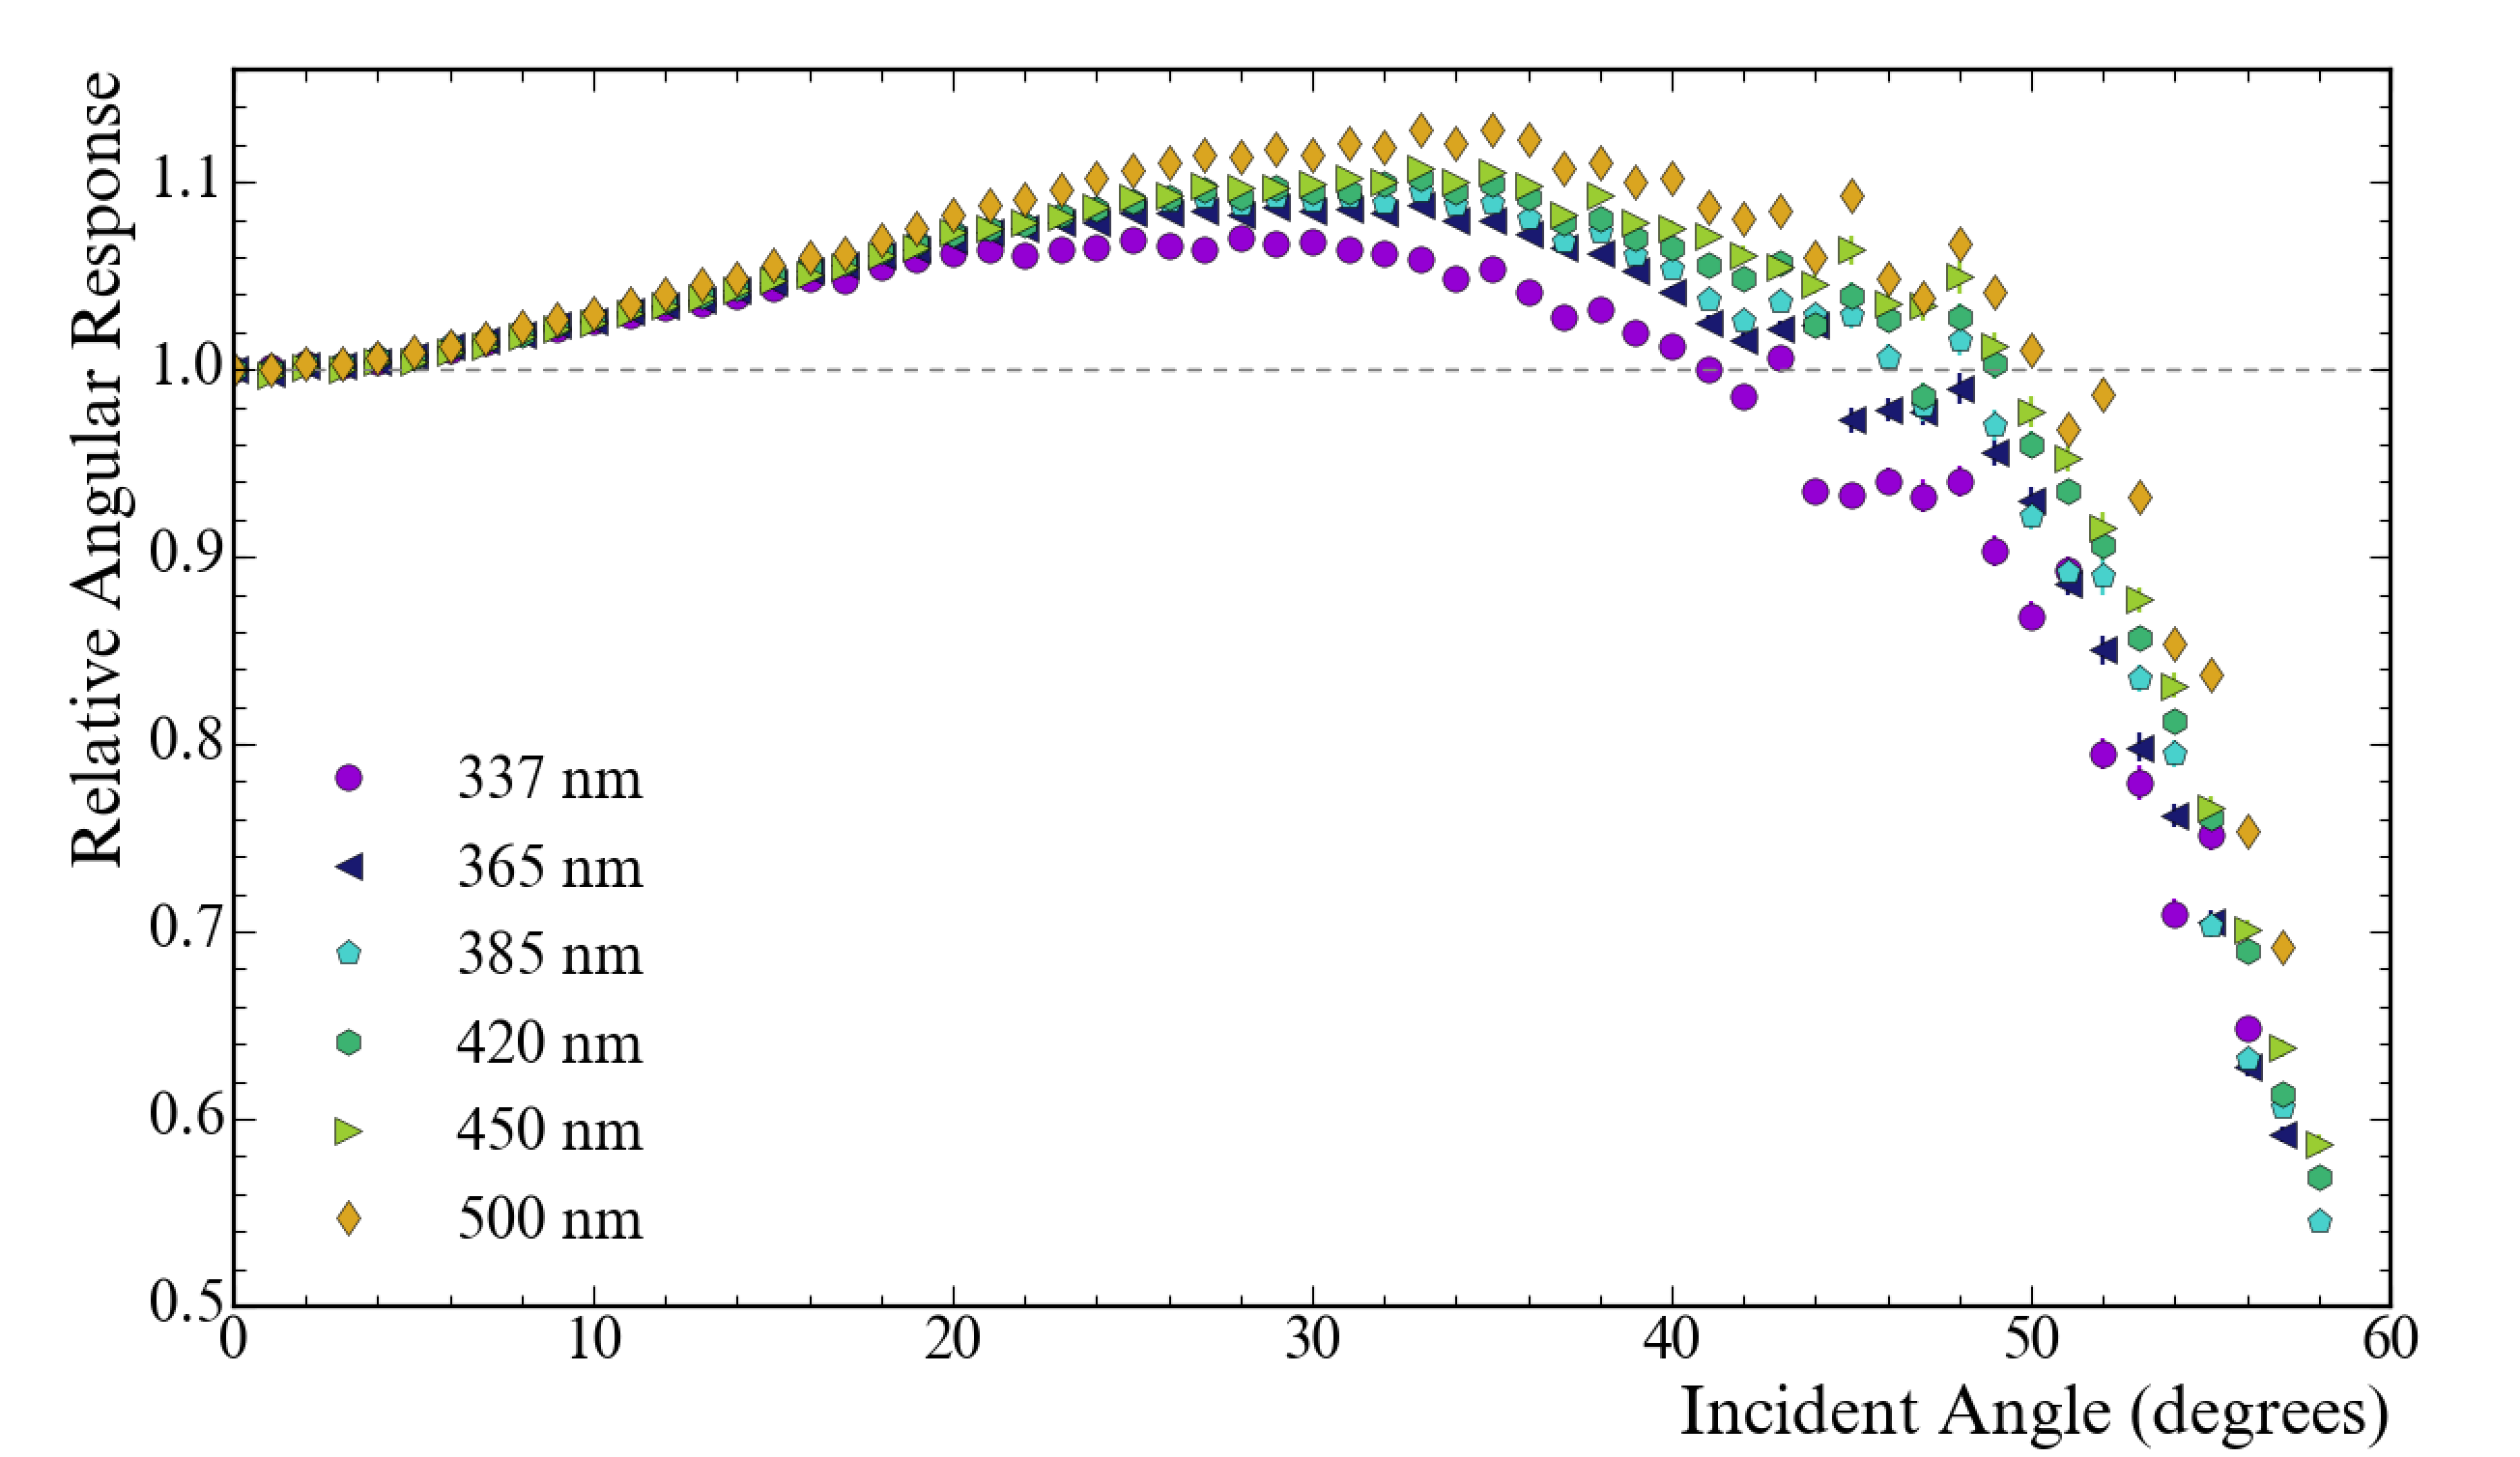
\includegraphics[width=0.95\textwidth]{2_Detector/Figs/PMTResponse.png}
        \caption{}
        \label{fig:pmt_angular_response}
    \end{subfigure}
    \caption[Diagram of the PMT and concentrator `bucket' used within SNO+; and plot of the measured relative angular response of the PMTs in SNO+]{\textbf{(a):} Diagram of the PMT and concentrator `bucket' used within SNO+, showing also the definition of the incidence angle. \textbf{(b):} Plot of the measured relative angular response of the PMTs in SNO+, as a function of both incidence angle and wavelength. Both figures taken from~\cite{andersonOpticalCalibrationSNO2021}.
    }
    \label{fig:pmt_optics}
\end{figure}

\nomenclature{\textbf{QE}}{Quantum efficiency (of a PMT)}
\nomenclature{\textbf{TTS}}{Transit time spread (of a PMT)}
% \nomenclature{\textbf{FWHM}}{Full-width at half-maximum (of a distribution)}
Once a photon is incident on the PMT's photocathode, it is possible for that photon to be absorbed and generate a photoelectron. The probability of this happening is governed by the photocathode's Quantum Efficiency (QE) at the photon's wavelength. In addition, the collection efficiency defines the probability that a generated photoelectron actually created a recorded signal. The combined measured efficiency of PMTs tested \textit{ex-situ} for SNO can be seen in Fig~\ref{fig:qe_pmts}. Once this photoelectron has been created, it is accelerated by an electric field within the PMT, onto the PMT's first dynode. The natural spread in drift times is known as the `Transit Time Spread' (TTS) of the PMTs: for SNO+, the RMS of the TTS for the R1408-type PMTs is $\sim\SI{1.7}{\ns}$~\cite{BOGER2000172}. % cite SNO-era papers
The collision of the photoelectron with the dynode generates further electrons, which collide with subsequent dynodes to generate a cascade that eventually produces an observable voltage signal.

\begin{figure}
    \centering
    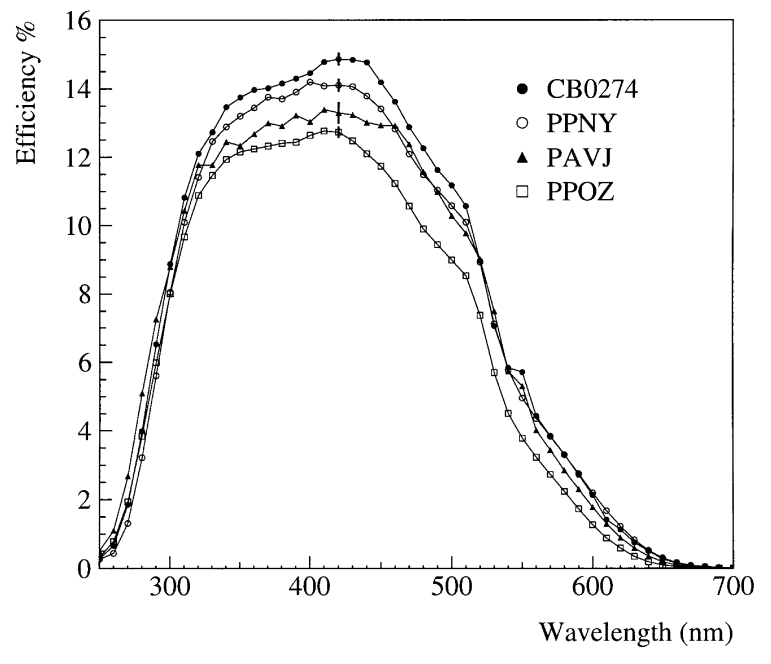
\includegraphics[width=0.7\textwidth]{2_Detector/Figs/efficiencies_PMTs_biller1999.png}
    \caption[Efficiencies of the R1408-type PMTs used as standard within SNO+]
    {Efficiencies of four R1408-type PMTs tested for calibration by~\cite{billerMeasurementsPhotomultiplierSingle1999}. % cite
    }
    \label{fig:qe_pmts}
\end{figure}

\nomenclature{\textbf{npe}}{Number of photoelectrons}
Finally, if multiple photons generate photoelectrons on the same PMT close enough in time, the amount of charge generated increases in proportion to the number of photoelectrons (npe). Much like with the transit time, the strength of the signal observed by the PMT is governed by a distribution, a function of the npe generated. Examples of these distributions can be seen in Fig.~\ref{fig:charge_dists_pmt}. % cite
The relatively large widths of these charge distributions precludes the ability to straightforwardly determine the npe purely from charge when the npe is small. To work around this, various techniques can be employed to try and estimate the npe in a given PMT --- an example of one such method can be seen in Section~\ref{sect:new_beam_profiles}.

\begin{figure}
    \centering
    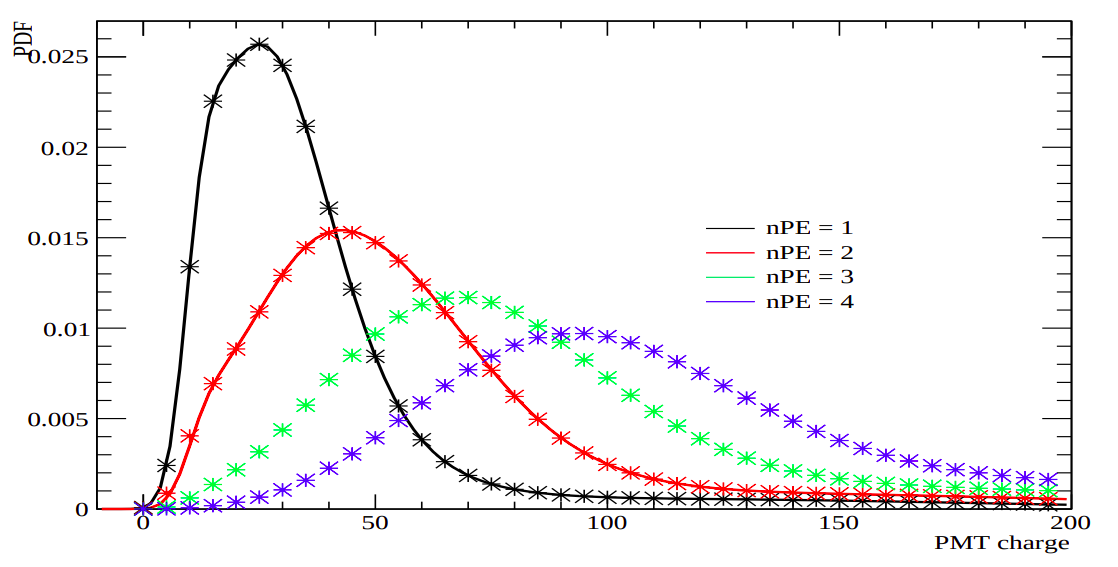
\includegraphics[width=0.8\linewidth]{2_Detector/Figs/charge_spectra_mod.png}
    \caption[Example charge spectra for a PMT as a function of the true npe generated]{Example charge spectra for a PMT as a function of the true npe generated. Figure taken from~\cite{dungerOccupancyAnalysisMultipleHit2016}. % cite whom?
    }
    \label{fig:charge_dists_pmt}
\end{figure}


    % \begin{itemize}
    %     \item Light gets detected via the PMTs. Note the existence of the PMT concentrators to maximise coverage within the AV, but minimise it in the external water: show the calibrated angular response.
    %     \item Remind reader that a PMT converts photons to photoelectrons with a certain quantum efficiency, dependent on the wavelength of light.
    %     \item The process of multiplying the signal induces a spread in the possible generated time of the voltage signal, known as the PMT's transit time spread.
    %     \item The PMT response is also weakly dependent on the number of photoelectrons generated; not enough to be able to confidently distinguish the npe under most circumstances.
    % \end{itemize}
    % [2 pages]
\subsection{Data Acquisition and Triggering}\label{sec:daq}
\nomenclature{\textbf{DAQ}}{Data acquisition (system)}
Once a signal reaches the cable attached to a PMT, it travels along up to the front-end electronics on the deck above the detector. The job of these electronics, known as the data acquisition (DAQ) and triggering system, is to convert raw electronic signals from the PMTs into recorded digital `events' that can be used for analysis. A schematic showing the setup of the electronics is shown in Fig~\ref{fig:tdaq_schematic}, with full details in~\cite{albaneseSNOExperiment2021}. % cite

\begin{figure}
    \centering
    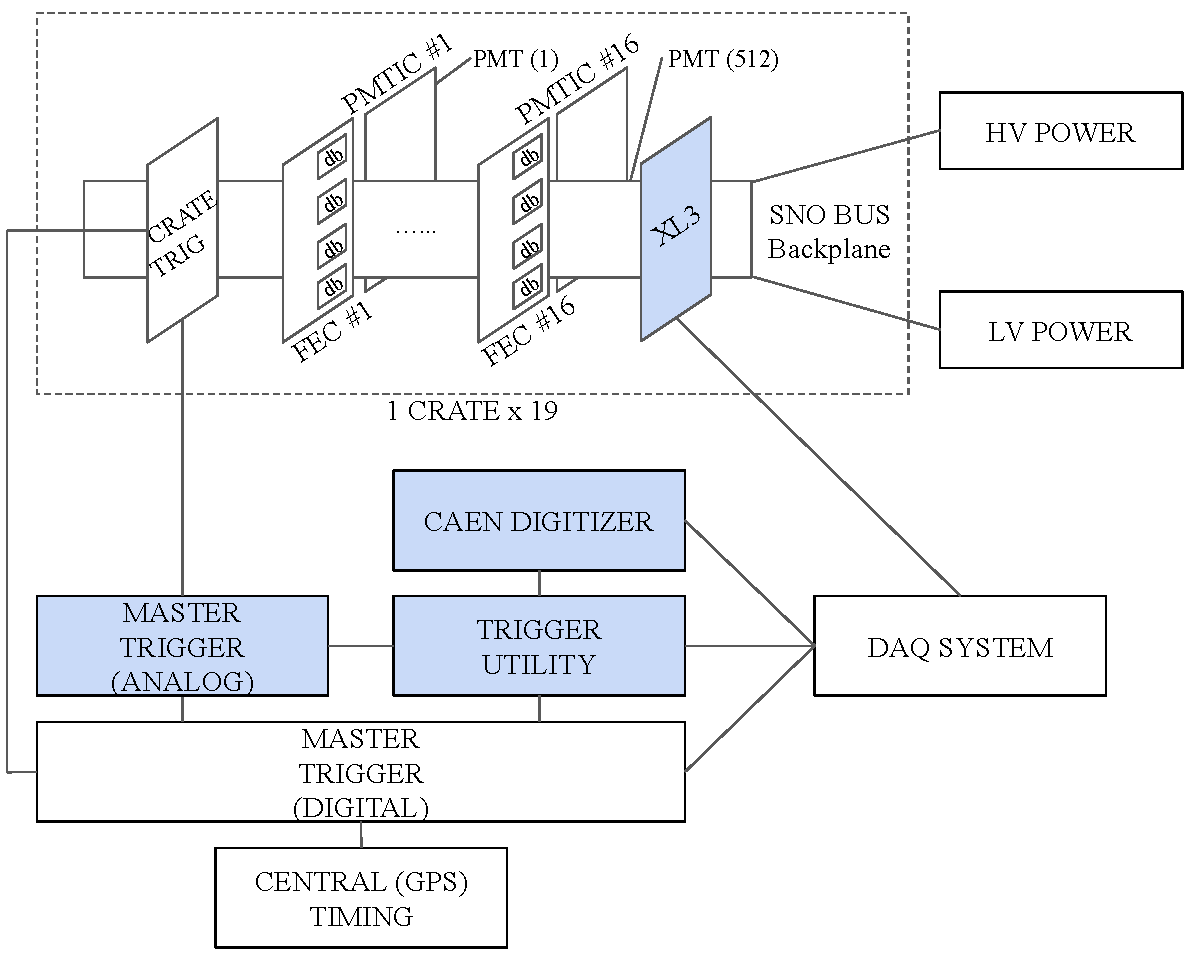
\includegraphics[width=0.7\linewidth]{2_Detector/Figs/electronics_diagram.pdf}
    \caption[Schematic of the front-end electronics used for data acquisition and triggering in SNO+]{Schematic of the front-end electronics used for data acquisition and triggering in SNO+, taken from and discussed in~\cite{albaneseSNOExperiment2021}. % cite
    }
    \label{fig:tdaq_schematic}
\end{figure}

\nomenclature{\textbf{PMTIC}}{PMT Interface Card}
\nomenclature{\textbf{DB}}{Daughter Board}
\nomenclature{\textbf{FEC}}{Front-End Card}
\nomenclature{\textbf{TAC}}{Time-to-amplitude Converter}
\nomenclature{\textbf{QHS}}{Charge with high gain over a `short' integration time (\SI{60}{\ns})}
\nomenclature{\textbf{QHL}}{Charge with high gain over a `long' integration time (\SI{390}{\ns})}
\nomenclature{\textbf{QLX}}{Charge with low gain over a `long' integration time (\SI{390}{\ns})}
A signal passes first through the PMT Interface Card (PMTIC), which then sends it through to one of the Daughter Boards (DBs) which are stored on Front-End Cards (FECs) within one of 19 electronic crates on deck. The DBs determine if the analogue signal along a given PMT channel has crossed a pre-defined charge threshold, at which point a `hit' is said to have been detected on that PMT's channel. When this occurs, the DB performs a set of important actions:
\begin{enumerate}
    \item Begins a timer for that channel, in the form of a Time-to-Amplitude Converter (TAC). TAC also corresponds to the resulting analogue voltage on the output of the TAC being measured.
    \item Begins integrating the total charge signal for that channel in three ways, known as QHS, QHL, and QLX. These correspond to using different integration times and gain settings.
    \item Generates trigger pulses for that channel for each available trigger type. Three main trigger signals are the `N20' (a square pulse for \SI{20}{\ns}), `N100' (a square pulse for \SI{100}{\ns}), and `ESUMHI' (a pulse copying the shape of the voltage signal for that channel).
\end{enumerate}

\nomenclature{\textbf{CTC}}{Crate Trigger Card}
\nomenclature{\textbf{MTC/A+}}{Analogue Master Trigger Card}
Whilst the TAC, QHS, QHL, and QLX are being calculated, the trigger signals from each channel are sent over to the Crate's Trigger Card (CTC), where the signals are then summed for each trigger type. These crate-level trigger signals are then sent over to the 7 detector-level Analogue Master Trigger Cards (MTC/A+), which further sum the signals by trigger type from all the crates in the detector. The combined N20 and N100 signals are proportional to the total number of hit PMTs within a \SI{20}{\ns} and \SI{100}{\ns} time window, respectively, whilst the total ESUMHI signal corresponds to the total charge seen over all the PMTs.

\nomenclature{\textbf{MTC/D}}{Digital Master Trigger Card}
\nomenclature{\textbf{GT}}{Global Trigger}
\nomenclature{\textbf{EXTA}}{External Asynchronous (Trigger)}
\nomenclature{\textbf{TUBii}}{Trigger Utility Board Mark ii}
If these trigger signals go above certain pre-defined thresholds, then a signal is sent for that trigger type to the Digital Master Trigger Card (MTC/D). The MTC/D receives all trigger signals from the detector, and if a given trigger type has been `masked in' (i.e. activated) the Card will generate a Global Trigger (GT) for the detector with a time stamp from its \SI{50}{\MHz} clock. Under certain circumstances, such as calibrations, a trigger signal can be generated externally and asynchronous to the MTC/D: these are `EXTA' triggers. Any such EXTA trigger signal is first handled by an electronics box named `TUBii' (Trigger Utility Board Mark ii), before then being passed onto the MTC/D. TUBii functionality will become relevant when discussing the calibration electronics described in Chapter~\ref{chap:smellie_hardware}.

\nomenclature{\textbf{ADC}}{Analogue-to-Digital Converter}
Once a GT signal is generated, it is then sent back to all the CTCs, which then orders the integration of time and charge to be stopped on all channels for that crate. The time and charge information that has been temporarily stored on each channel's CMOS chip on the FEC is then sent to the crate's `XL3' card, which packages the crate's raw information via ethernet over to a set of computers. The trigger signals for a triggered event are also digitised by a CAEN brand Analogue-to-Digital Converter (ADC), and sent to the same DAQ computers. The total window of time in which data is gathered from one GT signal is \SI{400}{\ns}, with data from up to \SI{180}{\ns} before and \SI{220}{\ns} after the GT has arrived. There is then a necessary `dead time' of \SI{420}{\ns} after a given GT has been given in which no further GTs can be made.

\nomenclature{\textbf{ZDAB}}{Zebra Database (file format)}
\nomenclature{\textbf{GTID}}{Global Trigger Identification number}
Finally, the raw data from the crates and trigger system arrives in a set of computers, which organise all of this into an individually-packaged `event', stored on disk in the `Zebra Database' (ZDAB) format. A given built event contains the TAC and charge information from each hit PMT, the CAEN digitised waveforms, a unique identifying number for that triggered event (the GTID), as well as the times from both the MTC/D's \SI{50}{\MHz} clock and a GPS-calibrated \SI{10}{\MHz} clock. The former time is used for measuring relative times between events whilst the latter is used for knowing the time of day of an event: both are used in Chapter~\ref{chap:solar_osc_analysis}.


    % \begin{itemize}
    %     \item Summarise how a PMT signal becomes digitised via the front-end electronics, briefly.
    %     \item Summarise the triggering system, as I'll have to describe in a later chapter how the SMELLIE hardware fits into this, especially as there have been ongoing SMELLIE triggering issues worth mentioning there!
    %     \item Note the information stored by an event: importantly for this thesis, the TAC and QHS per hit, the event's GTID as well as trigger time measured from the \SI{50}{\mega\Hz} clock. The latter is worth mentioning as this is how I determine time differences for my BiPo tagging in the solar analysis.
    %     \item Finally, note that these get written to file in the ZDAB format.
    % \end{itemize}
    % [3 pages]
\subsection{Operation of the Detector}\label{sec:detector_ops}
Control of the detector's DAQ system is handled through a custom-built GUI known as ORCA~\cite{howeSudburyNeutrinoObservatory2004}. %cite
This program allows operators of the detector to modify settings in the detector electronics at both a low- and high-level. It also allows operators to monitor the current status of the detector, such as voltage and current levels within each crate.

ORCA allows for the detector to have its data split into `runs' of different types. For the majority of the time, the detector is run in the `Physics' mode, with individual runs split into 1 hour periods. It is this data that is used for almost all high-level physics analyses, such as the one described in Chapter~\ref{chap:solar_osc_analysis}. To help with the movement and processing of data, runs of raw data are split into ZDAB files of maximum size \SI{1}{\giga\byte}. Because of this, the number of files generated per run is proportional to the trigger rate of the detector. In the current \SI{2.2}{\gpl} LAB-PPO scintillator phase under nominal conditions, the trigger rate is $\sim\SI{2.5}{\kilo\Hz}$, leading to 15 ZDAB files being generated per run of 1 hour in length.

Other detector run types include ones for detector maintenance, as well as for calibrations of various kinds. During certain calibration runs, data can be further split into `subruns' where necessary. This allows for data taken from a given calibration source to have the different settings used (e.g. different wavelength settings) all kept within one run, but still appropriately separated. Operation of specific calibration sources, including the one described in Chapter~\ref{chap:smellie_hardware}, can be performed through the ORCA GUI.


    % \begin{itemize}
    %     \item Detector electronics operated through ORCA; allows for different running modes, such as calibrations.
    %     \item Mention that data gets split into run and subruns.
    % \end{itemize}
    % [1 page]
\section{Detector Calibrations and Modelling}\label{sec:calibs_modelling}
Once the raw data from triggered events has been stored in files, certain extra steps must be taken before effective analysis of that data can be achieved. This section covers those steps.

\subsection{Detector Monitoring}
No data taken from the detector can reasonably be used for analysis unless its quality has been approved. This is done in a number of ways on SNO+. Firstly, a number of automated systems monitor all aspects of the detector, including voltage levels in the crates, trigger rates, as well as `slower' quantities such as the tensions on the ropes holding the AV in place. Problems in any of these measured parameters trigger an automatic alarm system, which notifies a human detector operator. A human detector operator monitors the detector whenever the detector is live.

\nomenclature{\texttt{RATDB}}{RAT Database}
In addition to systems that monitor whether anything has gone wrong, information about the state of the detector during each run is stored in a database known as \texttt{RATDB}. This information includes, amongst other things, a recording of which PMT channels have actually been raised to high voltage for that run, as well as any channels/cards/crates that have been flagged for having a known poor data quality (e.g. being overly noisy).


    % \begin{itemize}
    %     \item Detector's state is continuously monitored via a number of systems for data quality purposes, including a human detector `shifter'. This includes the alarm systems for the electronics and slow controls, and `nearline' monitoring of the detector status.
    %     \item CHS and CSS ensure only ``good'' channels used in any analysis.
    % \end{itemize}
    % [1 page]
\subsection{Electronic and PMT Calibrations}
\nomenclature{\textbf{ECA}}{Electronic Calibration}
\nomenclature{\textbf{PCA}}{PMT Calibration}
The lowest level of calibrations performed in SNO+ are the Electronic and PMT Calibrations: ECAs and PCAs, respectively. These calibrations allow conversion of the raw time and charge values recorded by the DAQ into quantities that can actually be used in analysis.

During an ECA, two main quantities are measured. Firstly, because of noise the integrated charge measured on each channel is offset by some amount. This offset, known as the `pedestal', is recorded for each channel. The other quantity is the `time slope' for each channel, which allows one to convert from the ADC TAC counts into an uncalibrated hit time of that channel's PMT. Both of these quantities are measured by sending external signals to channels in the crates, forcing them to start measuring TAC and charge even though no PMTs were actually hit. Running ECAs also allows any channels with unusual behaviour to be spotted, so that they are not used during analysis. ECAs are typically done on a fortnightly basis, or after maintenance to the DAQ system has been performed.

Using ECAs alone is not enough to have fully-calibrated time and charge data. The lengths of cables between PMTs and PMTICs are all slightly different, leading to differences in the so-called `cable delay' of each channel. This means that two PMTs that have a photoelectron generated at the same time can generate slightly different TAC values. Furthermore, because the start time of the TAC is determined by when the channel's signal goes above a constant threshold, if a signal is very large (e.g. when numerous photoelectrons have been generated on one PMT) then the start time of the TAC will be systematically earlier. This is known as the `time walk'. Both of these quantities get measured during PCAs.

\nomenclature{\textbf{ELLIE}}{Embedded LED/Laser Light Injection Entity}
\nomenclature{\textbf{TELLIE}}{Timing subsystem for ELLIE}
PCAs can be performed by either the Laserball or by the TELLIE calibration system. The Laserball is an \SI{11}{\cm} quartz sphere, filled with small glass beads suspended in silicone gel, which diffuses laser light that is sent into it~\cite{moffatOpticalCalibrationSudbury2001,andersonOpticalCalibrationSNO2021}. The result is a near-isotropic light source that can be deployed within the detector in different positions, via use of a series of ropes. The TELLIE system is a series of 92 optical fibres attached at various points of the PSUP, through which optical-wavelength light can be fired from LEDs. TELLIE is the Timing subsystem of the ELLIE calibration system: the Embedded LED/Laser Light Injection Entity. The other two fibre-based optical calibration subsystems, AMELLIE and SMELLIE, are introduced in Section~\ref{sec:eo_calibs}. For both the Laserball and TELLIE calibration systems, the cable delay and time walk are measured by firing light from the source at a known time and with a known hit occupancy, and observing when the signal arrives in each PMT channel.

On top of calibrating the PMT hit times, PCAs also further calibrate the charge information. In particular, the charge spectrum generated by a single photoelectron is determined for each channel. This allows us to convert the pedestal-corrected charge ADC counts into an approximate number of photoelectrons.

Using the data gathered from both ECAs and PCAs, the raw data stored in \texttt{ZDAB}s is processed into a new file format known as \texttt{RATDS} files. These files contain all the information of an event, but now the timing and charge information have been calibrated. It is this file type used in the optical calibration work of Chapters~\ref{chap:smellie_hardware}--\ref{chap:smellie_analysis}.

    % \begin{itemize}
    %     \item First main set of calibrations are the ECAs and PCAs. These help us convert raw electronic signal information from PMTs into `calibrated' hit times and charges. PCAs performed via TELLIE and the Laserball.
    %     \item These initial calibrations allow for the first two passes of data processing, resulting in a `RATDS' file format used in optical calibrations.
    %     \item No need for many details here; this is not a thesis on this topic!
    % \end{itemize}
    % [1 page]
\subsection{Energy and Optical Calibrations}\label{sec:eo_calibs}
The next stage of calibrating the detector is modelling its optical properties. These properties include all the processes covered in Section~\ref{sec:optical_processes}, such as scintillator emission, optical absorption, re-emission, and Rayleigh scattering.
This is crucial, as it allows us to reconstruct information about events within the detector.

\nomenclature{\textbf{AMELLIE}}{Attenuation Module for ELLIE}
\nomenclature{\textbf{SMELLIE}}{Scattering Module for ELLIE}
In addition to deployments of the Laserball (discussed in Section~\ref{sec:optical_processes}), two further calibration sources are used in SNO+ to measure properties of light propagation: AMELLIE and SMELLIE. These are the `Attenuation Module' and `Scattering Module' of the ELLIE calibration system. Like TELLIE, AMELLIE and SMELLIE consist of optical light sources that shine through optical fibres into the detector. The former uses LEDs from TELLIE, whilst the latter uses optical wavelength lasers. Despite the names both subsystems are similar enough that they are both capable of measuring attenuation and scattering within the detector. More details about the SMELLIE hardware can be read in Chapter~\ref{chap:smellie_hardware}.

\nomenclature{\textbf{AmBe}}{Americium-Beryllium radioactive source}
Another critical component of the detector to calibrate well is the energy response: given a specific amount of energy deposited in the water/scintillator, how many hits are observed? For this, a number of radioactive sources are used at a variety of energies. In the scintillator phase, there are three main sources. The first is an americium-beryllium (AmBe) source inherited from SNO~\cite{loachMeasurementFlux8B2008}, % SNO AmBe paper
which contains \ce{^{241}Am} that $\alpha$-decays. These $\alpha$ particles can be captured by the \ce{^{9}Be} within the source, leading to the emission of a neutron as well as production of a \ce{^{12}C} nucleus, which 60\% of the time is in  an excited state. When this excited state decays, a \SI{4.4}{\MeV} $\gamma$ is emitted promptly. Eventually the neutron is captured by hydrogen (typically) in the detector, leading to a characteristic \SI{2.2}{\MeV} delayed $\gamma$ being generated~\cite{albaneseSNOExperiment2021}. % cite detector paper
Both the prompt and delayed peak energies from the AmBe source can be used for energy calibration. In addition to this, one can calibrate the neutron detection efficiency with the AmBe source~\cite{loachMeasurementFlux8B2008}, % cite AmBe paper
which is important for the analysis of antineutrino IBD events. % CONFIRM IBD acronym in chapter 1

The second radioactive source is the \ce{^{16}N} deployable source, also originally used for SNO~\cite{dragowsky16NCalibrationSource2002}. % SNO N16 paper
The \ce{^{16}N} isotope $\beta$-decays to \ce{^{16}O}, with a distinctive \SI{6.1}{\MeV} $\gamma$ also being generated 66\% of the time. It is the $\gamma$ that can make it out to the detector, whilst the $\beta$ can be tagged by a block of scintillator and PMT held within the source container.

In theory, sources can be deployed both within the AV (`internally') and in the water shielding (`externally'). Both internal and external deployments were used for the optical calibration of the water phase with the Laserball~\cite{andersonOpticalCalibrationSNO2021}. Although external deployments during the scintillator phase with the Laserball, \ce{^{16}N}, and AmBe sources have been made, there have been no such internal source deployments. This is a result of the substantial work currently underway~\cite{valderLaserballCalibrationDevice} to overhaul the internal deployment hardware, in order to satisfy the much more stringent radiopurity requirements of the scintillator phase over the water phase.

Alongside these two deployed sources, a third kind of radioactive source has been used during the scintillator phase for energy calibration: the existing radioactive background spectra within the detector. Backgrounds such as \ce{^{14}C}, \ce{^{210}Po}, \ce{^{214}BiPo}, and \ce{^{208}Tl} all have distinctive energy spectra that can be observed in SNO+, and can be used to calibrate the scintillator's energy response. \ce{^{214}BiPo} events in particular have been used for energy scale calibration with the solar oscillation analysis, as discussed in Section~\ref{sec:exp_rates_constraints}.

    % \begin{itemize}
    %     \item After ECAs and PCAs, further calibration is necessary to accurately model the optical properties of the detector.
    %     \item Describe briefly the function of the Laserball, SMELLIE, and AMELLIE sources in optical calibration (can reference the water-phase optical calibration paper). Details of how each analysis works is obviously not needed here, especially not for SMELLIE as we have 3 chapters to go over that!
    %     \item AmBe and N16 sources provide further information for calibration
    %     \item In-situ backgrounds used for more calibration sources, especially for determining the light yield of the scintillator, and Birks' constant.
    % \end{itemize}
    % [2 pages]
\subsection{Event Reconstruction}\label{sec:ev_reco}
Once the detector has been calibrated, event `reconstruction' becomes possible. This is the process of deriving high-level physics quantities about a triggered event within the detector, based upon the calibrated hit information. In SNO+, our base assumption in most event reconstruction is that a triggered event was due to a single electron track. Reconstructing an event involves running a number of algorithms, which in the scintillator phase are together called the \texttt{ScintFitter}.

\nomenclature{\textbf{TOF}}{Time-of-flight (of a photon)}
The first critical pieces of information that get determined by \texttt{ScintFitter} are the event's position and time. The reconstructed position corresponds to the point in the detector where the triggered event most likely came from (assuming the event was approximately point-like in extent), whilst the reconstructed time is the starting emission time of the event, relative to the event's trigger time. The position of an event is critical to know, as far fewer background events occur near the centre of the detector compared to the edges. It is also important to know the emission time of an event, as this allows us to build the so-called `time residual' (\tres{}) distribution of an event. For a point-like physics event in the detector, \tres{} for a given PMT hit is defined as:
\begin{equation}
    \tres = t_{\mathrm{hit}} - t_{\mathrm{TOF}} - t_{\mathrm{emm}},
\end{equation}
where $t_{\mathrm{hit}}$ is the calibrated hit time of the PMT, $t_{\mathrm{TOF}}$ is the time one expects for light to travel directly from the reconstructed position to that PMT (the time-of-flight), and $t_{\mathrm{emm}}$ is the reconstructed emission time. The \tres{} distribution of hits in a given event can be very useful in understanding the physics of that event.

Whilst a number of algorithms have been developed for reconstructing position and time in SNO+, they all work on the same basic principle. Because of the spherical symmetry of the detector, if an event occurs at the centre of the detector one expects direct light to hit PMTs throughout the detector at the same time\footnote{It is possible for the centre of the AV and PSUP to not be completely aligned, i.e. there is an `AV offset'. Then, the spherical symmetry can be very slightly broken by refraction through the AV. Fortunately, this is accounted for when coordinating the position fitters.}.
However, if an event happens some distance away from the detector's centre then direct light will arrive at the PMTs it is closer to sooner. Therefore, by looking at the distribution of hit times for PMTs that were hit earliest as a function of the PMTs' positions in the detector (ignoring PMT hits that arrived much later, presumably because the photon paths were not direct) one can try and estimate where the position of the event was. Reconstructed positions and reconstructed times are linked by the time residual equation described above.

A likelihood-based approach is currently used to reconstruct position and time in SNO+. The algorithm endeavours to maximise the combined likelihood of the observed calibrated hit times of the hit PMTs, given proposed points in the four-dimensional (position, time) parameter space~\cite{jonesBackgroundRejectionNeutrinoless2011,coulterModellingReconstructionEvents2013,parkerMultiPDFMethodPosition2021}. % cite Multipath thesis
However, regardless of algorithm there are two factors that limit the position and timing reconstruction of an event. The TTS of the PMTs used as well as the speed of the scintillator emission timing defines the fundamental timescale --- and hence also length scale --- by which events can be reconstructed. Secondly, if more photons are able to generate prompt hits in the detector from a given event, then more information can be used to determine the position and time. Under current conditions, a \SI{2.5}{\MeV} event in the centre of the detector will have a position resolution of \SI{100}{\mm}~\cite{parkerRecoordinatingScintEffectiveSpeedMultiPDF2023}. % TODO & cite Will's recoordination!

The other critical piece of reconstructed event information is the event's energy. In energy reconstruction, the particle is assumed to be an electron, and the energy corresponds to the kinetic energy of the electron. By consequence, events due to $\alpha$-decay will obtain reconstructed energies well below the actual energy of the $\alpha$ particle, because of scintillator quenching (see Section~\ref{sec:scintillation} for details).

\nomenclature{\texttt{nhit}}{Number of PMT hits in an event}
At its simplest, assuming that an event is from an electron of moderate energy (e.g. at \SI{2.5}{\MeV}), then we can expect the number of PMT hits observed to be directly proportional to the energy of the event. Given that the number of hits observed in an event (called the \texttt{nhit}) is governed by a Poisson distribution, then the uncertainty in energy will just be proportional to the square root of the number of hits. As a result, the reconstructed energy resolution in SNO+ is determined by the scintillator's light yield and absorption length, as well as the coverage and QE of the PMTs.

There are second-order corrections to the energy reconstruction that need to be considered to minimise bias. At high energies, many PMTs will have had multiple photoelectrons generated, so merely using the \texttt{nhit} will give an underestimate of the true energy. Also, the detection efficiency of photons is non-uniform as a function of position in the detector. The current energy reconstruction algorithm used within SNO+ attempts to deal with all of these effects~\cite{mottramUpdatedFunctionalForm2015,kroupovaImprovingSensitivityNeutrinoless2020}. % cite energy reco info

After position, time, and energy reconstruction, \texttt{ScintFitter} calculates a number of additional quantities, known as classifiers. These describe a wide number of properties about an event, often using the derived \tres{} distribution of an event as the basis for classification. Some examples of classifiers used in analysis are discussed in Section~\ref{sec:background_processes}.

All Physics data runs, as well as certain calibration data such as AmBe and \ce{^{16}N}, have the \texttt{ScintFitter} algorithm run over it after having been processed for time and charge calibration. This results in what is known as a fully-processed \texttt{RATDS} file, as well as a new file type known as an \texttt{ntuple}. This latter file type has much of the hit-level information removed, and contains only event-level information such as the reconstructed energy and position. Because these files are much smaller, they are the ones typically used in the high-level physics analyses on the experiment, such as the one described in Chapter~\ref{chap:solar_osc_analysis}.


    % \begin{itemize}
    %     \item Once detector is calibrated, event reconstruction becomes possible. Describe main assumption of a SNO+ event: we assume a single-site electron event.
    %     \item Briefly describe the basics of how energy, position, and time reconstruction works, as this is needed for the solar analysis chapter. Mention existence of direction fitting in scintillator!
    %     \item `Physics' runs have their events reconstructed in a third pass of data processing, resulting in a `fully-processed' RATDS file as well as a simplified NTUPLE file used in high-level physics analyses (such as my solar analysis).
    % \end{itemize}
    % [2 pages]
\subsection{Event Simulation}\label{sec:ev_simulation}
\nomenclature{\texttt{RAT}}{Reactor Analysis Tool}
\nomenclature{\texttt{MC}}{Monte Carlo}
Simulations of events in SNO+ are performed using the software \texttt{RAT}~\cite{albaneseSNOExperiment2021}. % cite
Built on the \texttt{GEANT4} particle physics software framework, \texttt{RAT} is capable of simulating all aspects of the physics of an event within the detector via a Monte Carlo (MC) approach. This includes any particle physics that defines an event's generation, propagation and interactions of those particles in the detector media, the generation of light by both scintillation and Cherenkov processes, the propagation of that light, as well as the detection of that light by PMTs and simulation of the expected DAQ response. \texttt{RAT} is then used to process both simulation and data in the same way. In addition to being highly customisable, \texttt{RAT} can use the \texttt{RATDB} tables generated from a given data run when simulating to try and match those particular run conditions as closely as possible. \texttt{RAT} also offers a suite of tools to assist with analysis of data. The software is constantly being updated with new features --- the work done in this thesis uses \texttt{RAT} versions between 6.18.8 and 7.0.14, inclusive.

% {
%     \color{blue}
%     \begin{itemize}
%         \item Briefly describe overview of RAT software: not only provides the software by which the above data processing occurs, but allows for a GEANT4-based simulation of events in the detector. This simulation includes all parts of the physics described in Section~\ref{sec:event_journey}, including particle and nuclear physics interactions, optical photon creation and propagation, signal generation and event building based on simulated triggers of the electronics. These simulated events then get processed in the same manner as actual data is.
%     \end{itemize}
%     [1 page]
%     [24 PAGES TOTAL]
% }